
% Chapter 

%\chapter{Quantitative Analysis of Thesis reflexivity}{Analyse de la réflexivité} % Chapter title
\chapter{Analyse réflexive}


\markboth{\thechapter\space Réflexivité}{\thechapter\space Réflexivité}


\label{app:reflexivity} % For referencing the chapter elsewhere, use \autoref{ch:name} 

%----------------------------------------------------------------------------------------


Nous avons vu tout au long de ce travail le rôle crucial d'une réflexivité dans la démarche de recherche. Celle-ci a pu jouer pour la définitions des objets ou les questions posées, concrètement dans les travaux directement basés sur un travail de terrain, ou dans l'élaboration de théories ayant un aspect récursif. Sans prétendre avoir exhaustivement construit un ``méta-point de vue'' comme préconisé par~\cite{morin1991methode} pour la construction d'une pensée complexe, nous suggérons avoir apporté des éléments de réponse de manière préliminaire.


Nous proposons ici, en guise de ``méta-conclusion'', de mener une analyse quantitative pour la réflexivité, en appliquant les méthodes développées à notre travail lui-même. Nous menons dans un premier temps l'analyse du paysage scientifique à partir du corpus de notre bibliographie, puis analysons dans un second temps l'évolution de la connaissance produite en termes de projets et de domaines de connaissance.


Cette démarche est particulièrement originale puisqu'il n'existe à notre connaissance pas de monographie incluant explicitement sa propre analyse par des outils quantitatifs. Nous prenons le parti d'une utilisation plus systématique de ce genre de démarche, pour encourager le développement d'une connaissance de second ordre.


%%%%%%%%%%%%
\section{Hypernetwork analysis}{Analyse par hyperréseau}


Nous appliquons ici la méthodologie par réseau de citation et réseau sémantique développée en Chapitre~\ref{ch:modelinginteractions}. Le corpus initial est constitué de l'ensemble de notre bibliographie\footnote{Figée au 27/11/2017, et disponible à \url{https://github.com/JusteRaimbault/CityNetwork/raw/master/Models/Reflexivity/data/CityNetwork_20171127.bib}.} qui comporte 834 références.


\subsection{Citation Network}{Réseau de citation}

Nous reconstruisons le réseau de citation à profondeur deux à partir de ce corpus initial, et obtenons un réseau conséquent ($\left|V\right| = 177428$, $\left|E\right| = 203317$), de degré moyen $2.29$ (degré moyen entrant $1.15$). Le coeur du réseau, constitué des sommets de degré supérieur ou égal à 2 pour la plus grande composante connexe (qui couvre 98\% du réseau), est de taille $\left|V\right| = 19714$ et $\left|E\right| = 47348$.


% IGRAPH 9dd0bbb DN-- 177428 203317
% mean(degree(citation))
%[1] 2.291825
% mean(degree(citation,mode="in"))
% [1] 1.145913

% citationcore
%IGRAPH c617c58 DN-- 19714 47348 -- 


Une détection de communautés par algorithme de Louvain donne une modularité dirigée de 0.74 pour 19 communautés de taille supérieure à 10. Nous interprétons les communautés par les étiquettes suivantes données en Table~\ref{tab:app:reflexivity:citationcoms}. Nous retrouvons des domaines directement couverts et utilisés dans notre travail (Systèmes Urbains, Modèles Spatiaux de Croissance Urbaine), et d'autres voisins évoqués mais pas directement utilisés (Fractales, Economie Géographique, Space Syntax).


%Chaos, Economie Géographique, Systèmes Urbains, ABM, Datamining, Réseaux, Statistiques Spatiales, Fractales, Lois Puissance, Economie Géographique Évolutionnaire, Epistémologie Quantitative, Modèles de Croissance Urbaine Spatialisés, Complexité, LUTI, Physique des Villes, Données Spatio-temporelles, Réseaux Biologiques, Space Syntax, VGI.


%%%%%%%%%%%%%
\begin{table}
\apptabcaption{\label{tab:app:reflexivity:citationcoms}}{\textbf{Communautés de citation.} La taille des communautés est donnée en proportion de la taille du coeur du réseau.\label{tab:app:reflexivity:citationcoms}}
\begin{tabular}{|l|l|}
\hline
Communauté & Taille \\ \hline
Economic Geography & 12.4 \% \\
Power Laws & 9.1 \% \\
Networks & 7.92 \% \\
Spatial Urban Growth Models & 7.67 \% \\
Physics of Cities & 7.43 \% \\
ABM & 7.37 \% \\
Complexity & 7.19 \% \\
LUTI & 7.16 \% \\
Urban Systems & 5.15 \% \\
Spatial Statistics & 5.13 \% \\
Evolutionary Economic Geography & 5.03 \% \\
Spatio-temporal data & 3.18 \% \\
Datamining & 2.81 \% \\
Quantitative Epistemology & 2.43 \% \\
Space Syntax/Procedural modeling & 2.43 \% \\
Fractals & 2.02 \% \\
VGI & 1.8 \% \\
Biological Networks & 1.33 \% \\
Chaos & 0.624 \% \\\hline
\end{tabular}
\end{table}
%%%%%%%%%%%%


%%%%%%%%%%%%
\begin{figure}
	%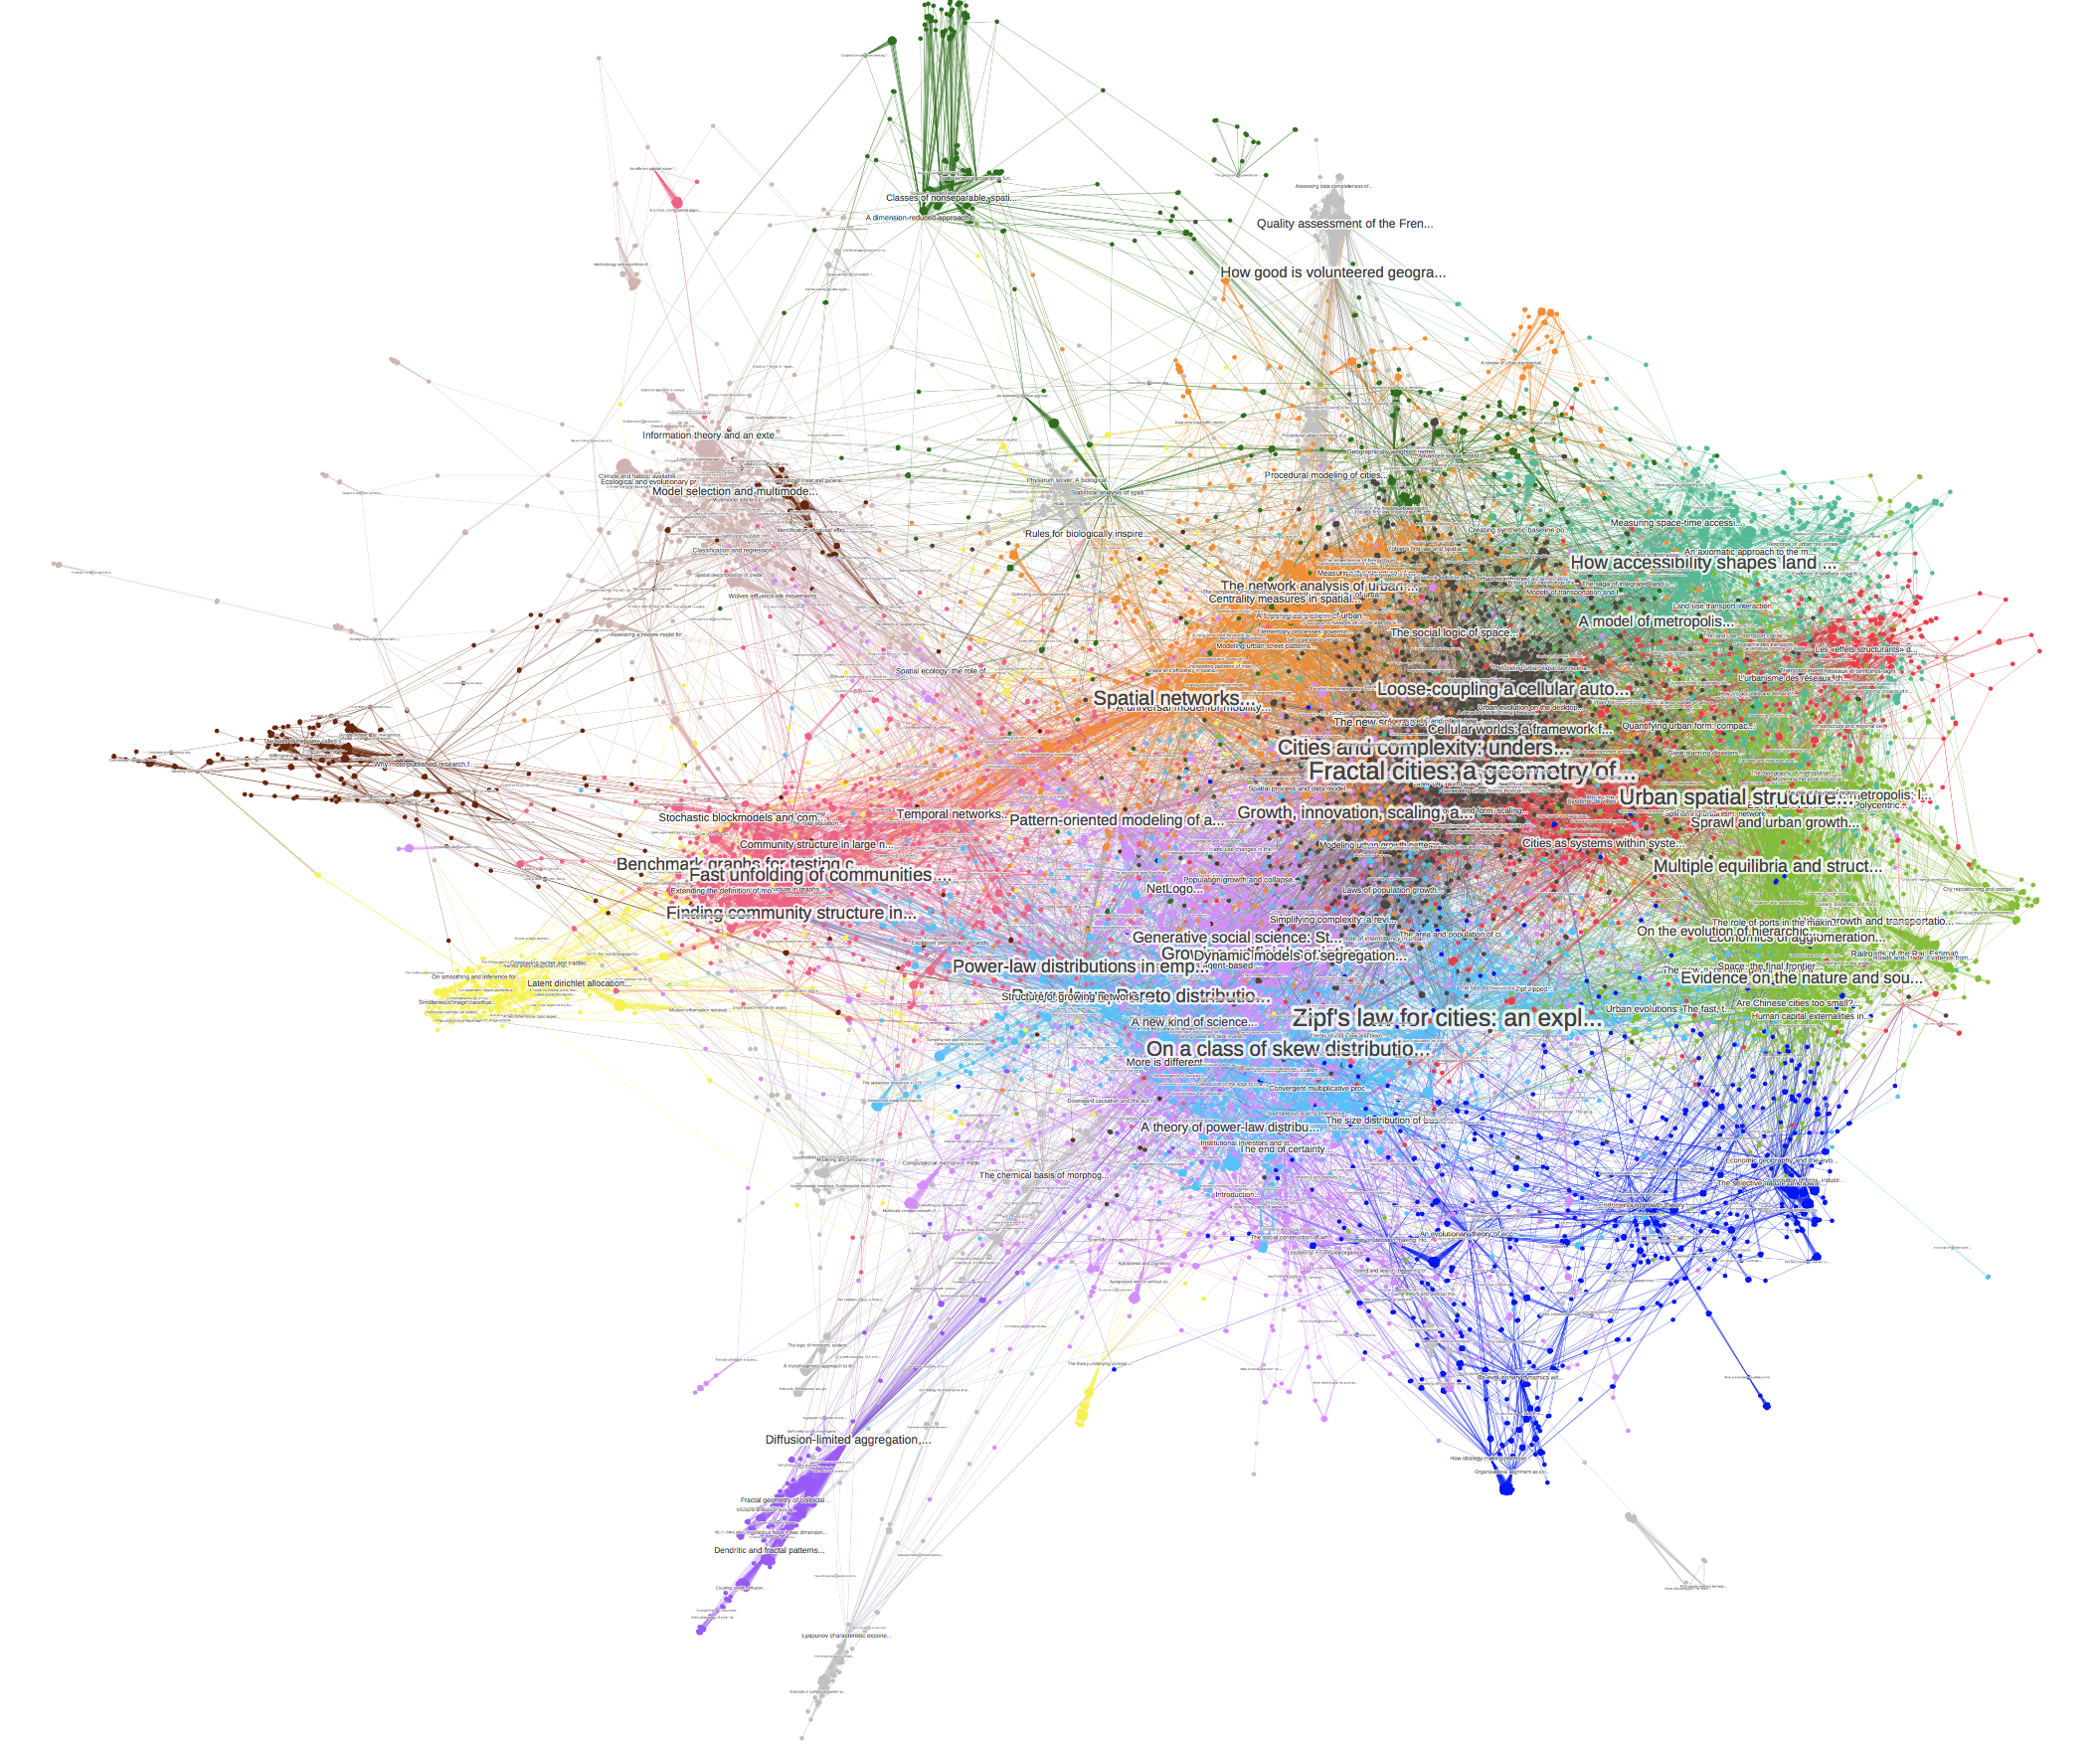
\includegraphics[width=\textwidth]{Figures/Reflexivity/citcore.png}
	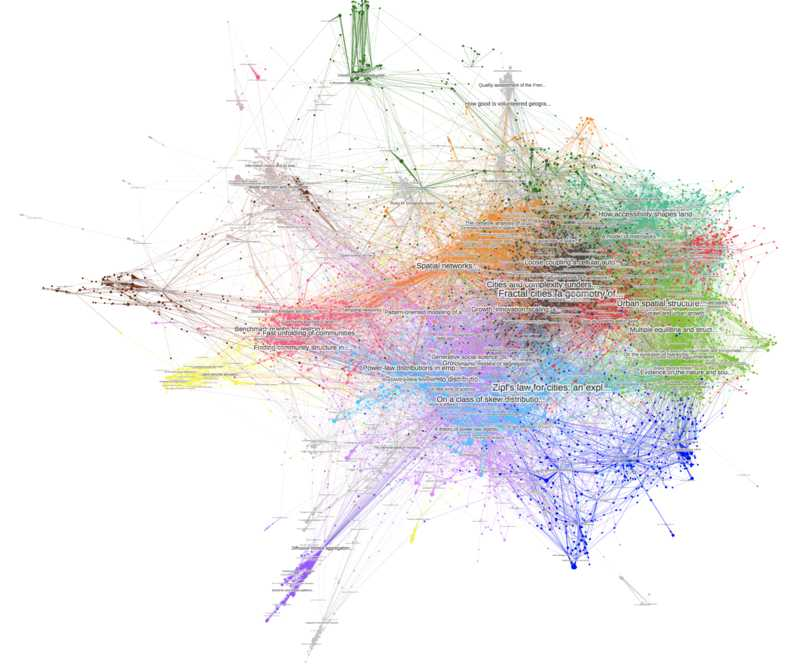
\includegraphics[width=\linewidth]{Figures/Final/F-reflexivity-citnw.jpg}
	\appcaption{\textbf{Citation network.}\label{fig:app:reflexivity:citnw}}{\textbf{Réseau de citation.} Nous visualisons uniquement le coeur du réseau, constitué ici des noeuds de degré supérieur ou égal à 2. Le réseau est spatialisé par algorithme Force Atlas 2. La taille des labels est proportionnelle au degré des noeuds, et la couleur donne la communauté.\label{fig:app:reflexivity:citnw}}
\end{figure}
%%%%%%%%%%%%

Le réseau de citation est visualisé en Fig.~\ref{fig:app:reflexivity:citnw}. Le positionnement des communautés est très instructif pour situer notre travail, qui forme des ponts entre différents domaines selon le point de vue choisi. Si nous prenons le parti des systèmes urbains, la communauté correspondante (en rouge) fait le pont entre modèles LUTI (turquoise) et modèles de croissance urbaine (noir) d'une part, et économie géographique (en vert). Si on se place du point de vue des modèles de simulation (communauté ABM, violet), le lien est fait entre Lois Puissances (bleu clair) et les réseaux et réseaux spatiaux (magenta et orange). Des communautés annexes se rattachent à la périphérie : Epistémologie Quantitative (jaune) est proche de l'analyse de réseau, tandis que l'analyse des processus spatio-temporels (vert foncé) est relativement indépendante. Les communautés dans lesquelles nos modèles peuvent être classifiés de manière thématique (modèles de croissance et systèmes urbains) sont situées au coeur de la partie compacte du réseau : cela confirme que les directions explorées ne sont pas périphériques, et que l'ensemble des domaines principaux périphériques évoqués étaient ``nécessaires'' au sens d'une forte connexion entre communautés ici.



%%%%%%%%%%%%
\subsection{Semantic Network}{Réseau sémantique}

% kminopt=0;kmaxopt=500;freqminopt=0;freqmaxopt=10000;ethopt=5

Après collecte des résumés, nous obtenons 91412 références sur lesquelles il est possible de procéder à l'analyse sémantique. La construction du réseau de co-occurrences brut, en filtrant les liens de poids inférieur à 5, et pour un nombre de mots-clés $K_W = 50000$, donne un réseau sémantique avec $\left|E\right|\simeq 16\cdot 10^6$. L'analyse de sensibilité aux paramètres de filtrage nous suggère de choisir $k_{min} = 0$, $k_{max}=500$, $f_{max} = 10000$, $\theta_w = 5$, ce qui fournit un réseau sémantique de taille $\left|V\right| = 37482$ et $\left|E\right| = 218926$, avec 26 communautés et une modularité de $0.78$. Les communautés principales peuvent être labellisées comme : toxicologie, chimie, sciences politiques, écologie théorique, systèmes urbains, soutenabilité, économie de l'innovation, analyse spatiale, physiologie, physique, réseaux, bio-anthropologie, santé, statistiques, microbiologie, transports, réseaux biologiques, géographie de la santé, botanique, évolution, écologie, génétique.

% 'toxicology','chemistry','political science','theoretical ecology','urban systems (french)','sustainibility','innovation economics','maup','physiology','NA','physics', 'networks','bioanthropology','health','statistics','microbiology', 'transportation','biological network','copyrights','publication','health geography','botanics','evolution','ecology','formulas','genetics')

Il est moins évident d'utiliser ce découpage pour comprendre notre travail, en comparaison au réseau de citation, puisque des domaines lointains (toxicologie, chimie, physiologie, botanique) se retrouvent en nombre relativement faible dans notre corpus de citation (provenant de citation commune sur la morphogenèse ou l'écologie par exemple) mais forment ensuite des communautés particulièrement isolées dans le réseau sémantique. Nous donnons en Fig.~\ref{fig:app:reflexivity:interdisc} la distribution des interdisciplinarités sémantiques par communautés de citation. À l'exception de l'économie géographique évolutionnaire qui est relativement plate (et donc assez cloisonnée) et de l'information géographique volontaire (VGI) qui présente un pic à 0 (attendu d'un domaine si spécifique), les communautés de citation ont fondamentalement le même profil d'interdisciplinarité.


%%%%%%%%%%%%
\begin{figure}
	%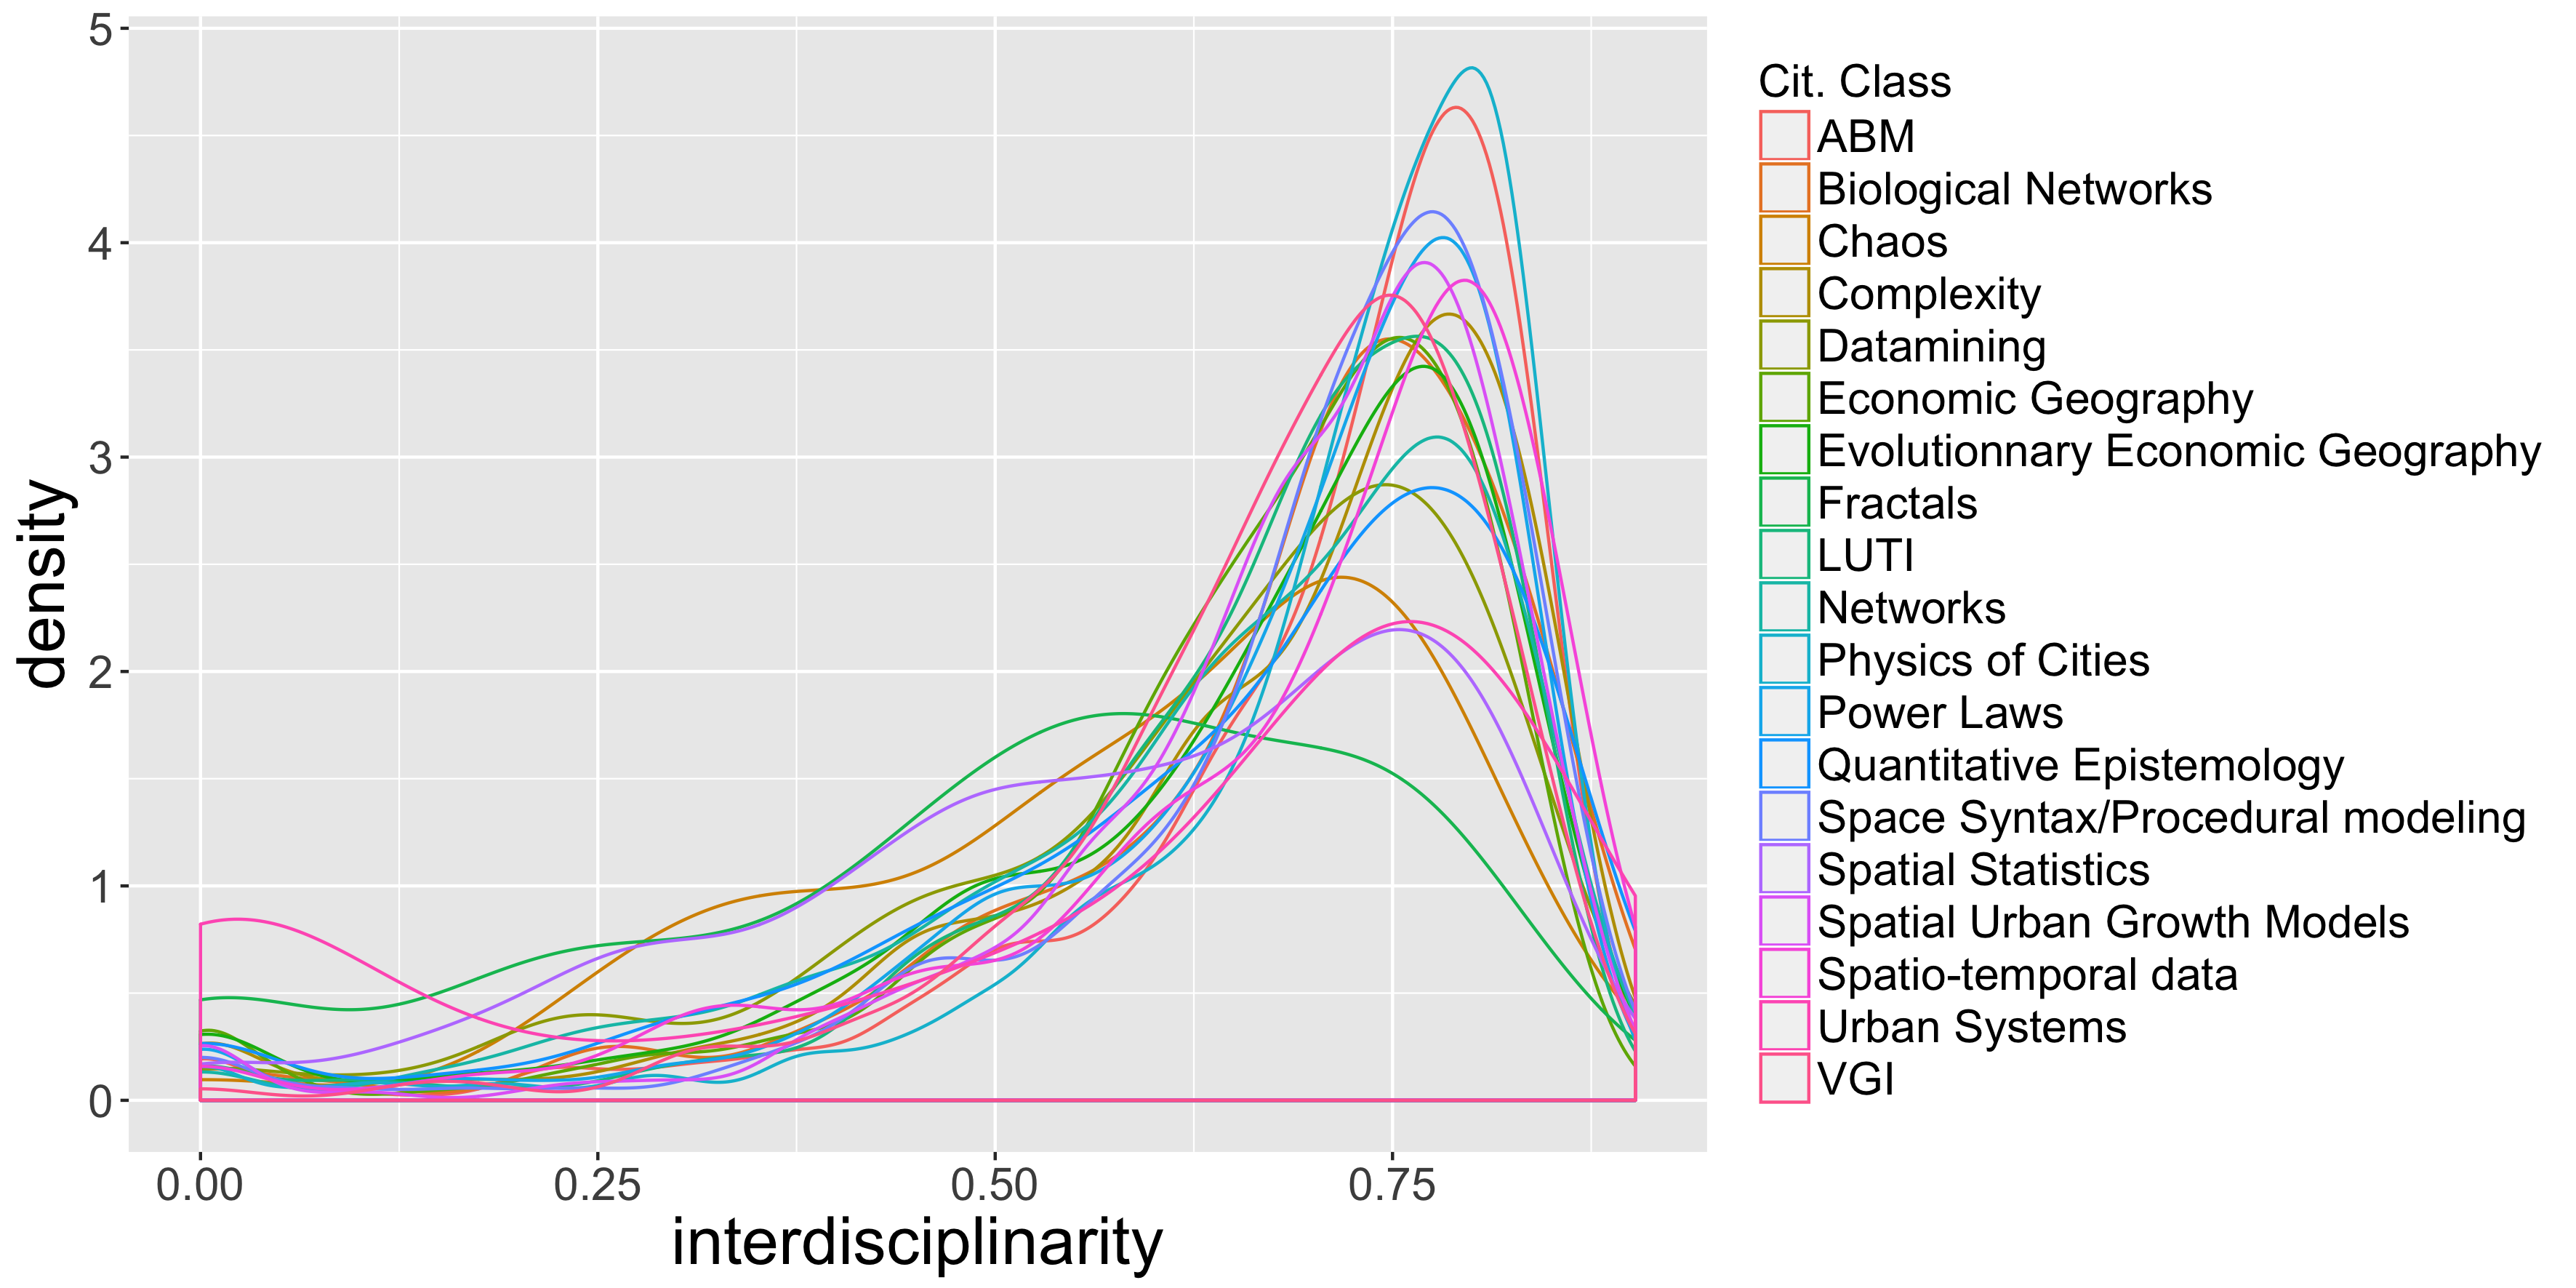
\includegraphics[width=\linewidth]{Figures/Reflexivity/interdisciplinarities.png}
	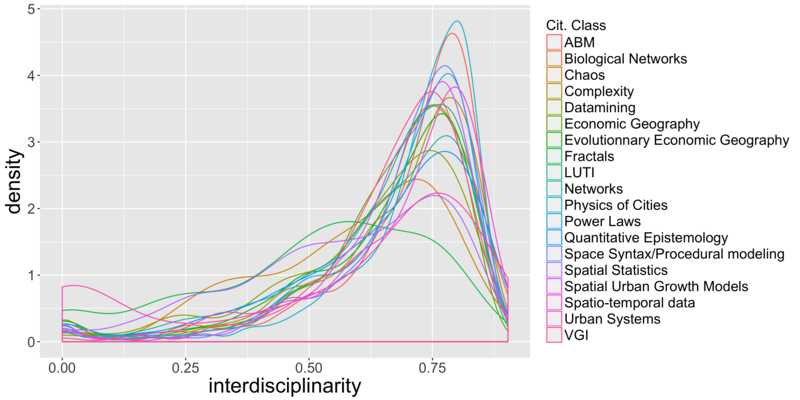
\includegraphics[width=\linewidth]{Figures/Final/F-reflexivity-interdisc.jpg}
	\appcaption{\textbf{Distribution of interdisciplinarities.}\label{fig:app:reflexivity:interdisc}}{\textbf{Distribution des interdisciplinarités par communauté de citation.}\label{fig:app:reflexivity:interdisc}}
\end{figure}
%%%%%%%%%%%%








%%%%%%%%%%%%
\section{Interaction between projects}{Interaction entre projets}


Nous proposons ici de quantifier l'évolution des différents projets et de leur interactions, ainsi que des domaines de connaissance associés. Un tableau du temps passé sur chaque projet, à la demi-heure près, a été tenu entre le 16/02/2015 et le 16/02/2018\footnote{Celui-ci est disponible à \url{https://github.com/JusteRaimbault/CityNetwork/raw/master/Docs/Organisation/Projects.ods}. Pour les analyses ici, nous utilisons la version figée au 02/12/2017}. Un projet est défini comme une entité minimale cohérente, soit par sa thématique (par exemple : modèle de morphogenèse de~\ref{sec:densitygeneration}) soit par son contenu (cas d'études, théorie géographique). Ceux-ci ayant été défini au cours du temps, certains se recoupent ou sont précurseurs d'autres : nous leur avons donc associé une classification a posteriori sous forme de ``macro-projets'' qui correspondent globalement à l'articulation finale. Nous leur attribuons également un domaine de connaissance majoritaire\footnote{Tout en sachant qu'il existe un biais non-négligeable dans le fait d'attribuer un domaine unique à un projet, puisque les domaines sont généralement intimement liés au coeur même de la production de connaissance. La contrainte de captation des données pousse toutefois à cette segmentation relativement réductionniste.} et la section principale de ce mémoire auxquels ils se rattachent.


La liste des projets est donnée en Table~\ref{tab:app:reflexivity:projects}, avec le macro-projet, le domaine et connaissance et le temps cumulé. La Fig.~\ref{fig:app:reflexivity:time} donne la répartition temporelle selon ces différentes modalités, dans le temps. Nous confirmons une organisation non-linéaire, la plupart des projets et chapitres étant menés en parallèle. Par exemple, le chapitre~\ref{ch:mesocoevolution} a fait l'objet d'une première exploration préliminaire dans les premiers mois, puis une résurgence à la convergence lorsque la maturité intellectuelle a été acquise. Les méthodes ponctuent régulièrement la répartition, mais culminent juste avant la première moitié. Les projets de modélisation, comme l'empirique, sont également régulièrement répartis, tandis que le conceptuel prend plus de place à la fin, ce qui confirme que celui-ci nécessite les autres domaines et une réflexion approfondie.


%%%%%%%%%%%%%
\begin{table}
	\apptabcaption{\label{tab:app:reflexivity:projects}}{\textbf{Descriptif des projets.} La section renvoie à la partie du mémoire où le projet est principalement utilisé. Des tâches génériques globales ne sont pas prises en compte dans le cumul par chapitre (Memoire : écriture de ce document ; Academic : vie académique ; Bibliography : lectures générales).\label{tab:app:reflexivity:projects}}
\begin{tabular}{|l|l|l|l|l|}
\hline
Projet & Macro-projet & Section & Domaine & Time (h) \\\hline
CaseStudies & Thematic & \ref{sec:casestudies} & Empirical & 5.5 \\
Modelography & QuantEpistemo & \ref{sec:quantepistemo} & Empirical & 20 \\
QuantEpistemology & QuantEpistemo & \ref{sec:quantepistemo} & Empirical & 32\\
MacroCoEvol & MacroCoEvol & \ref{sec:macrocoevol} & Modeling & 72 \\
SpatioTempCausality & CausalityRegimes & \ref{sec:causalityregimes} & Methods & 37.5 \\
Entretiens & Thematic & \ref{app:sec:interviews} & Data & 13 \\
MesoCoEvol & MesoCoEvol & \ref{sec:mesocoevolmodel} & Modeling & 60.5 \\
Fieldwork & Thematic & \ref{sec:qualitative} & Empirical & 27.5 \\
EnergyPrice & Empirical & \ref{sec:energyprice} & Empirical & 72.5 \\
Morphogenesis & Morphogenesis & \ref{sec:interdiscmorphogenesis} & Conceptual & 24.5 \\
NetworkNecessity & InteractionGibrat & \ref{sec:interactiongibrat} & Modeling & 158 \\
Memoire & Memoire & - & Conceptual & 489.5 \\
SpatialStatistics & CausalityRegimes & \ref{sec:causalityregimes} & Methods & 44 \\
BPCaseStudy & CausalityRegimes & \ref{sec:casestudies} & Empirical & 12 \\
Perspectivism & Epistemology & \ref{sec:knowledgeframework} & Conceptual & 8.5 \\
RealEstate & CausalityRegimes & \ref{sec:casestudies} & Empirical & 18 \\
Theory & Thematic & \ref{sec:networkterritories}, \ref{sec:theory} & Conceptual & 136\\
CorrelatedSyntheticData & Methods & \ref{sec:correlatedsyntheticdata} & Methods & 128 \\
MediationEcotox & Methods & \ref{app:sec:mediationecotox} & Methods & 59 \\
DensityGeneration & DensityGeneration & \ref{sec:densitygeneration} & Modeling & 84.5 \\
PatentsMining & Methods & \ref{app:sec:patentsmining} & Methods & 349.5 \\
CyberGeo & Methods & \ref{app:sec:cybergeo}, \ref{app:sec:cybergeonetworks} & Methods & 332 \\
SpaceMatters & Methods & \ref{sec:computation} & Methods & 100.5 \\
NetworkDensityStatistics & Empirical & \ref{sec:staticcorrelations} & Empirical & 176.5\\
NetLogoUtils & Tools & - & Tools & 10 \\
StochasticUrbanGrowth & Methods & \ref{app:sec:stochurbgrowth} & Methods & 13 \\
TransportationEquilibrium & Empirical & \ref{sec:transportationequilibrium} & Empirical & 56.5 \\
BiologicalNetwork & MesoCoEvol & \ref{sec:networkgrowth} & Modeling & 5 \\
Discrepancy & Methods & \ref{app:sec:robustness} & Methods & 54 \\
Governance & Governance & \ref{sec:lutecia} & Modeling & 228 \\
SyntheticData & Methods & \ref{sec:densitygeneration} & Methods & 99 \\
Reproduction & MacroCoEvol & \ref{sec:macrocoevolexplo} & Modeling & 46 \\
AlgorithmicReview & QuantEpistemo & \ref{sec:quantepistemo} &  Empirical & 75.5 \\
Tools & Tools & - & Tools & 137 \\
Academic & Acad & - & NA & 1388 \\
Bibliography & Biblio & - & Conceptual & 312 \\
\hline
\end{tabular}
\end{table}
%%%%%%%%%%%%%




%%%%%%%%%%%%
\begin{figure}
	%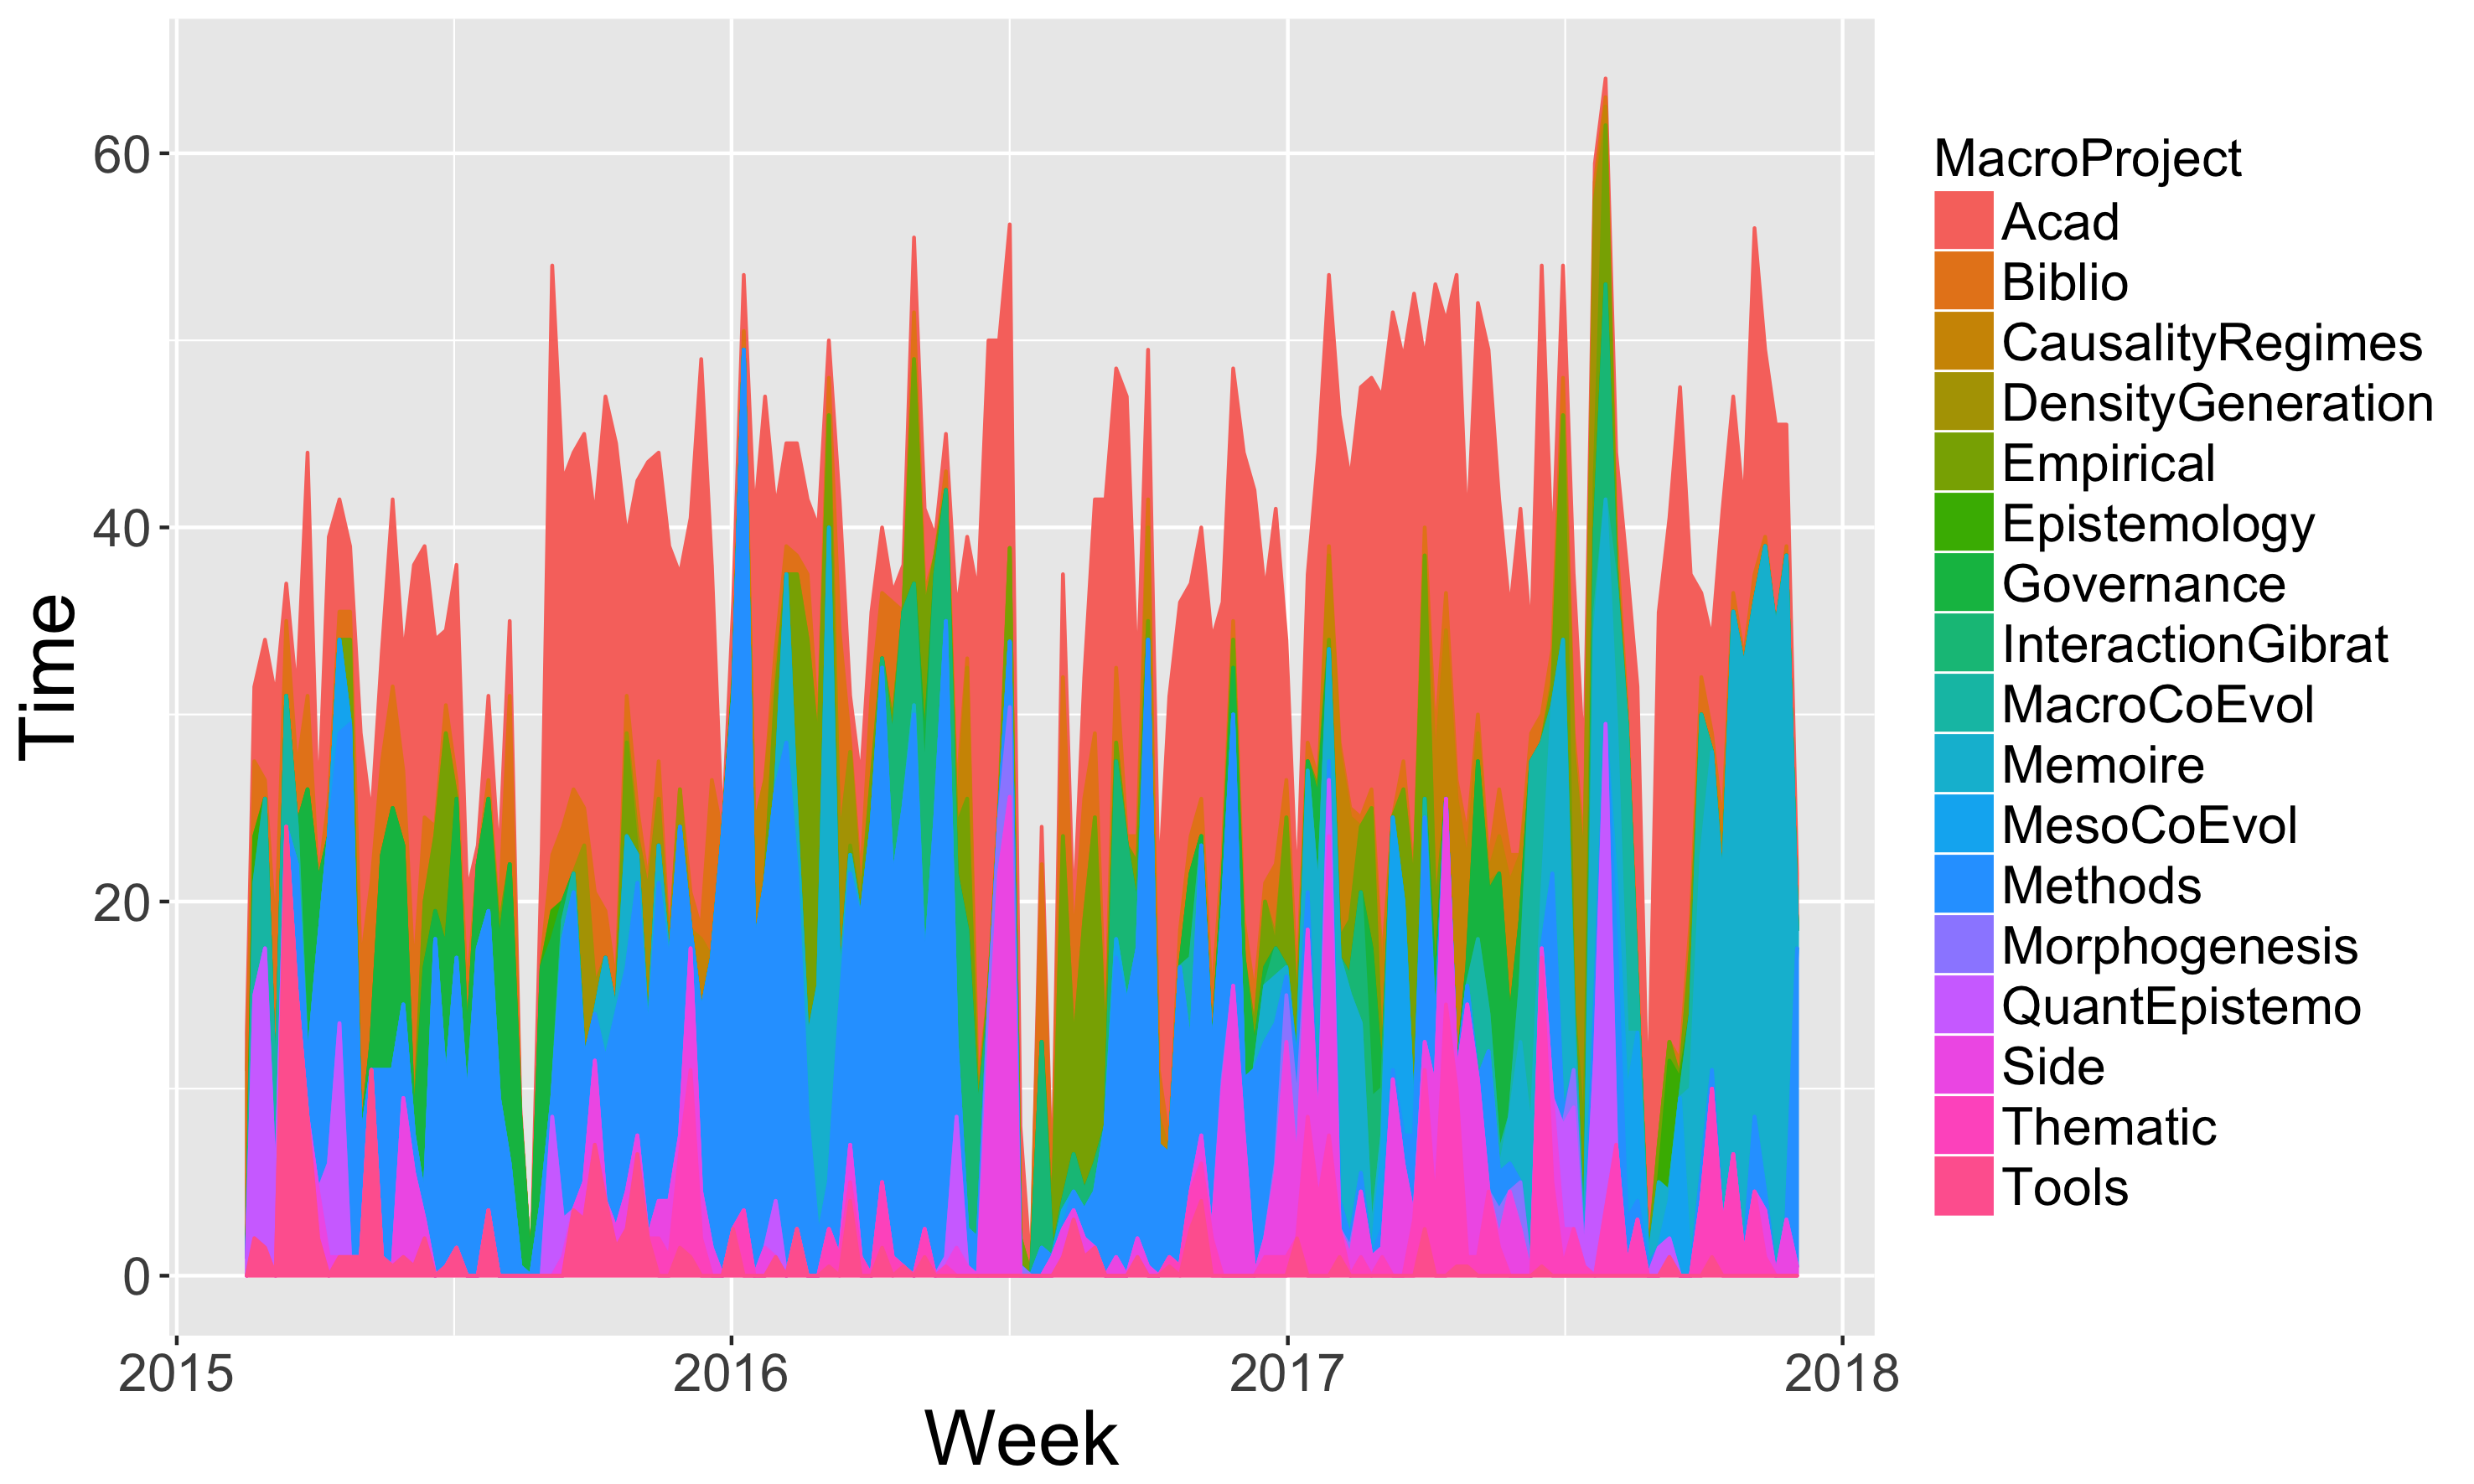
\includegraphics[width=\linewidth]{Figures/Reflexivity/weekly-macroproj.png}
	%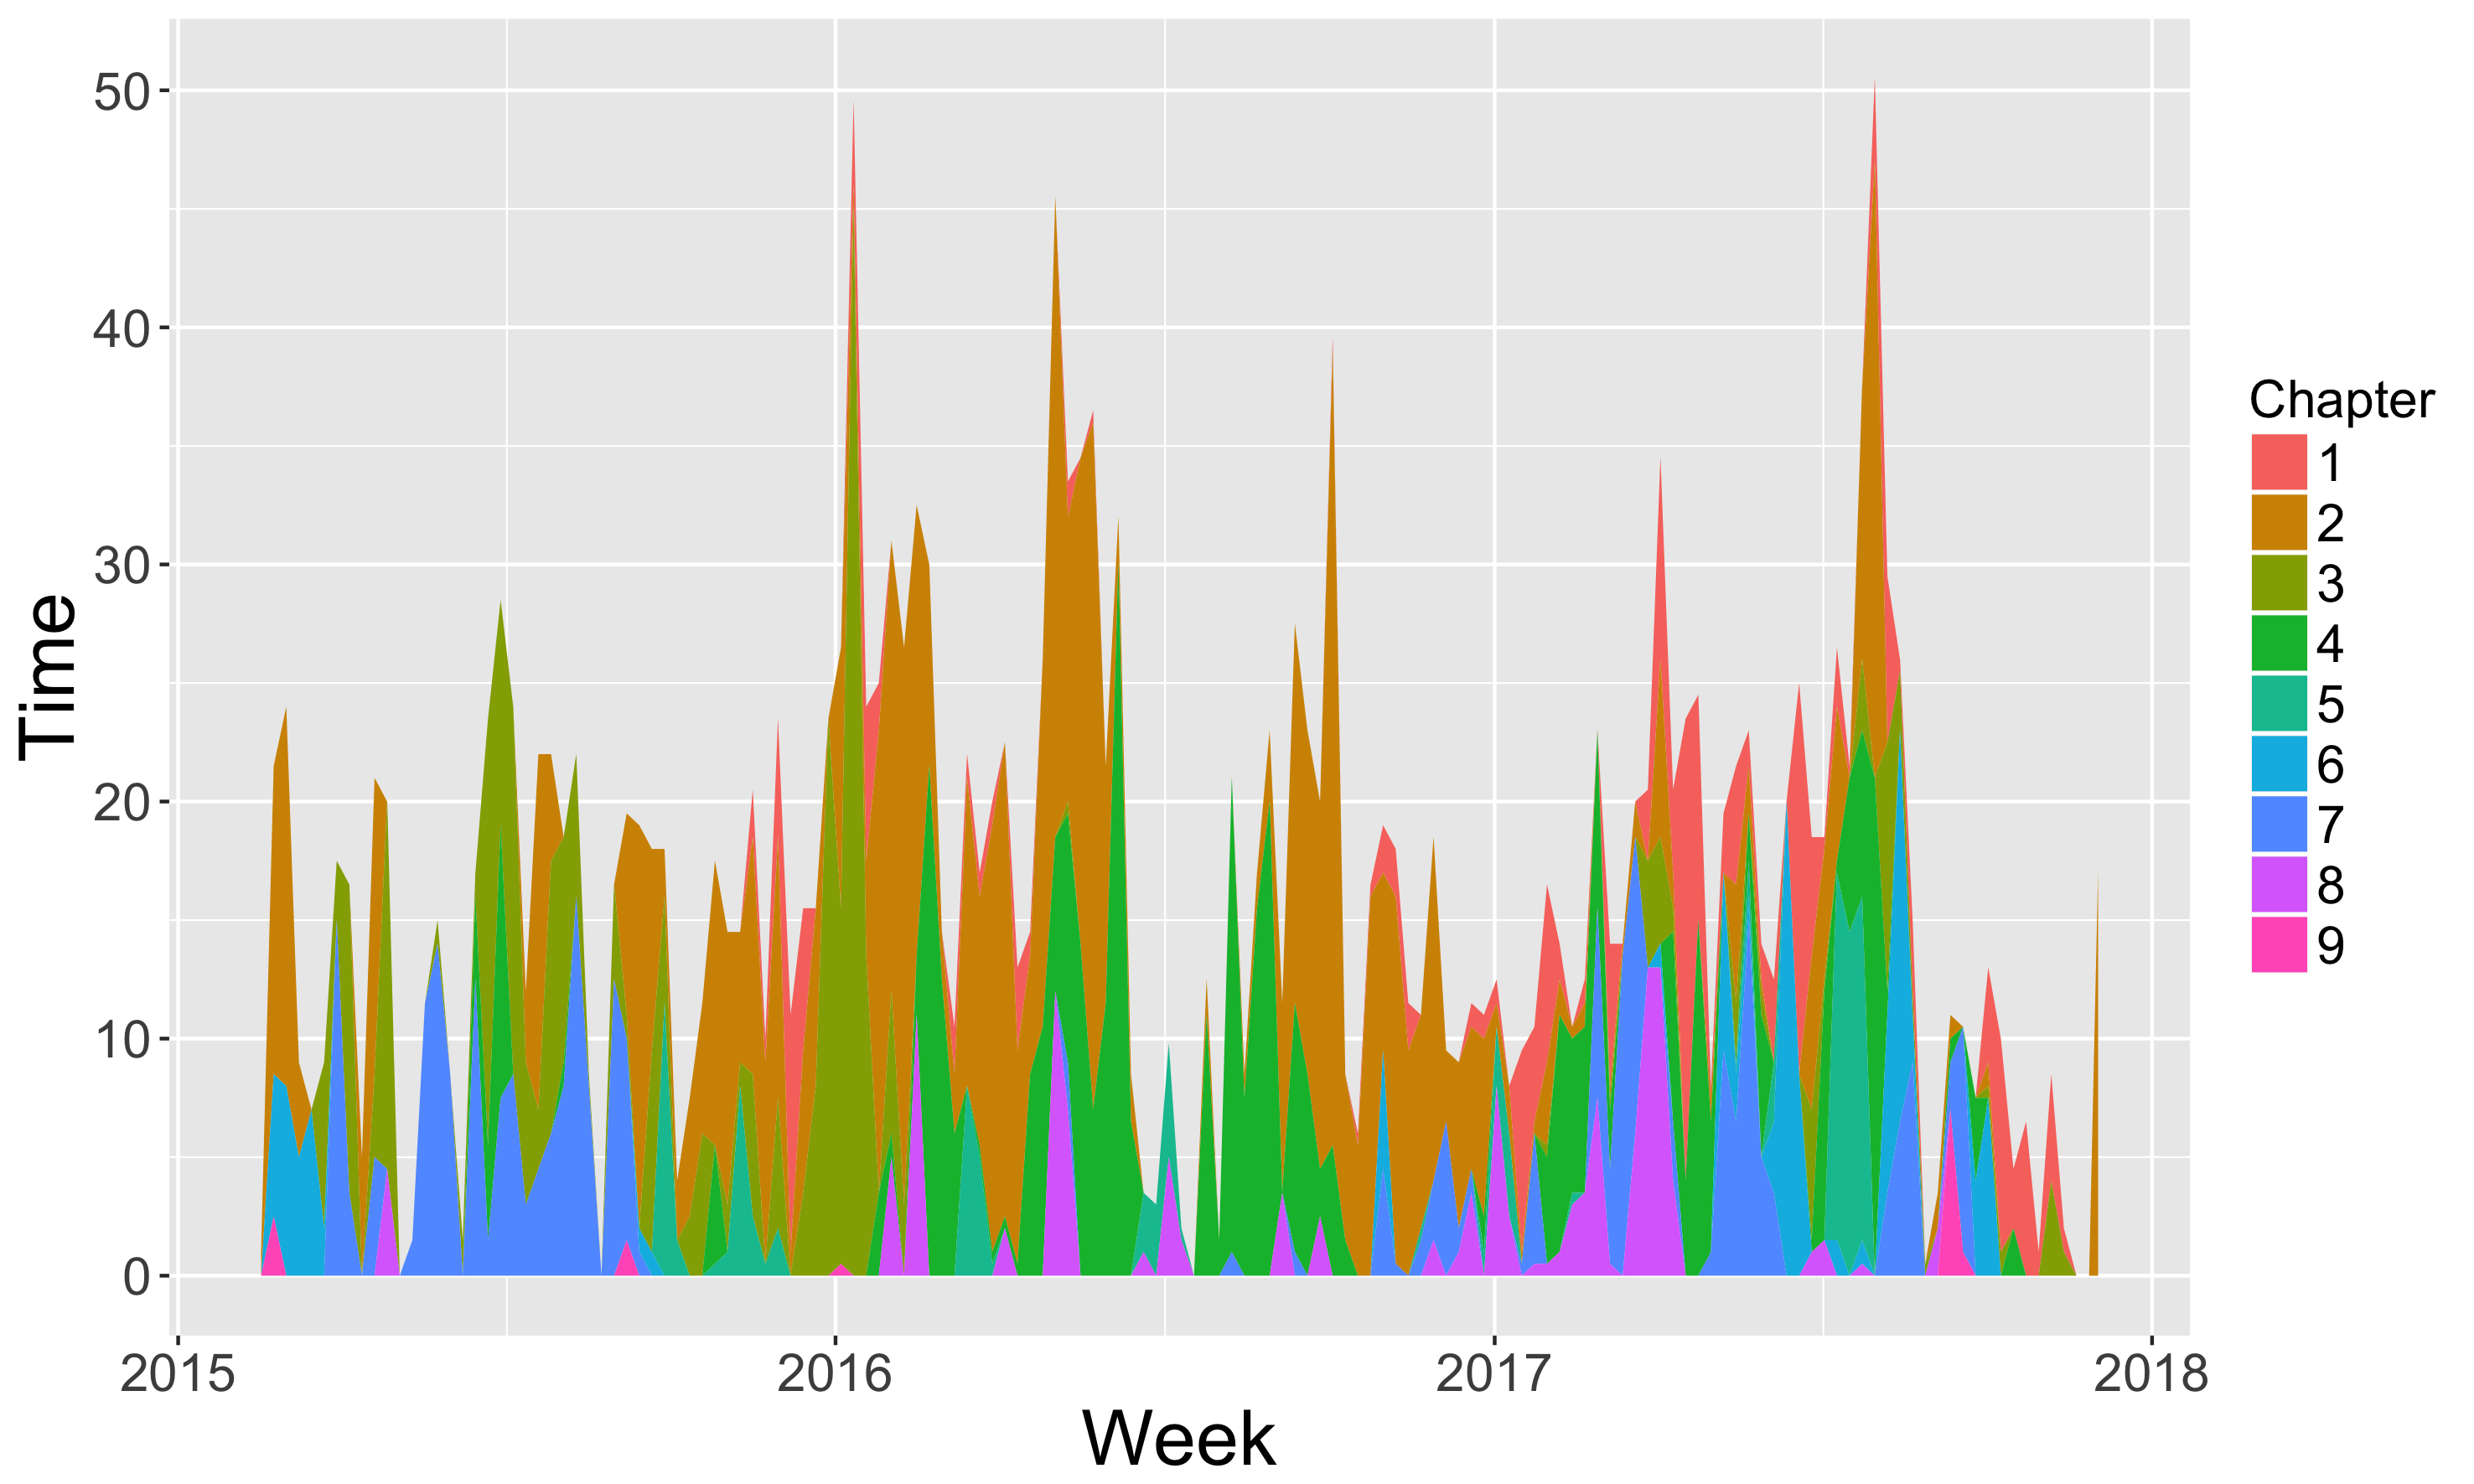
\includegraphics[width=\linewidth]{Figures/Reflexivity/weekly-chapter.png}
	%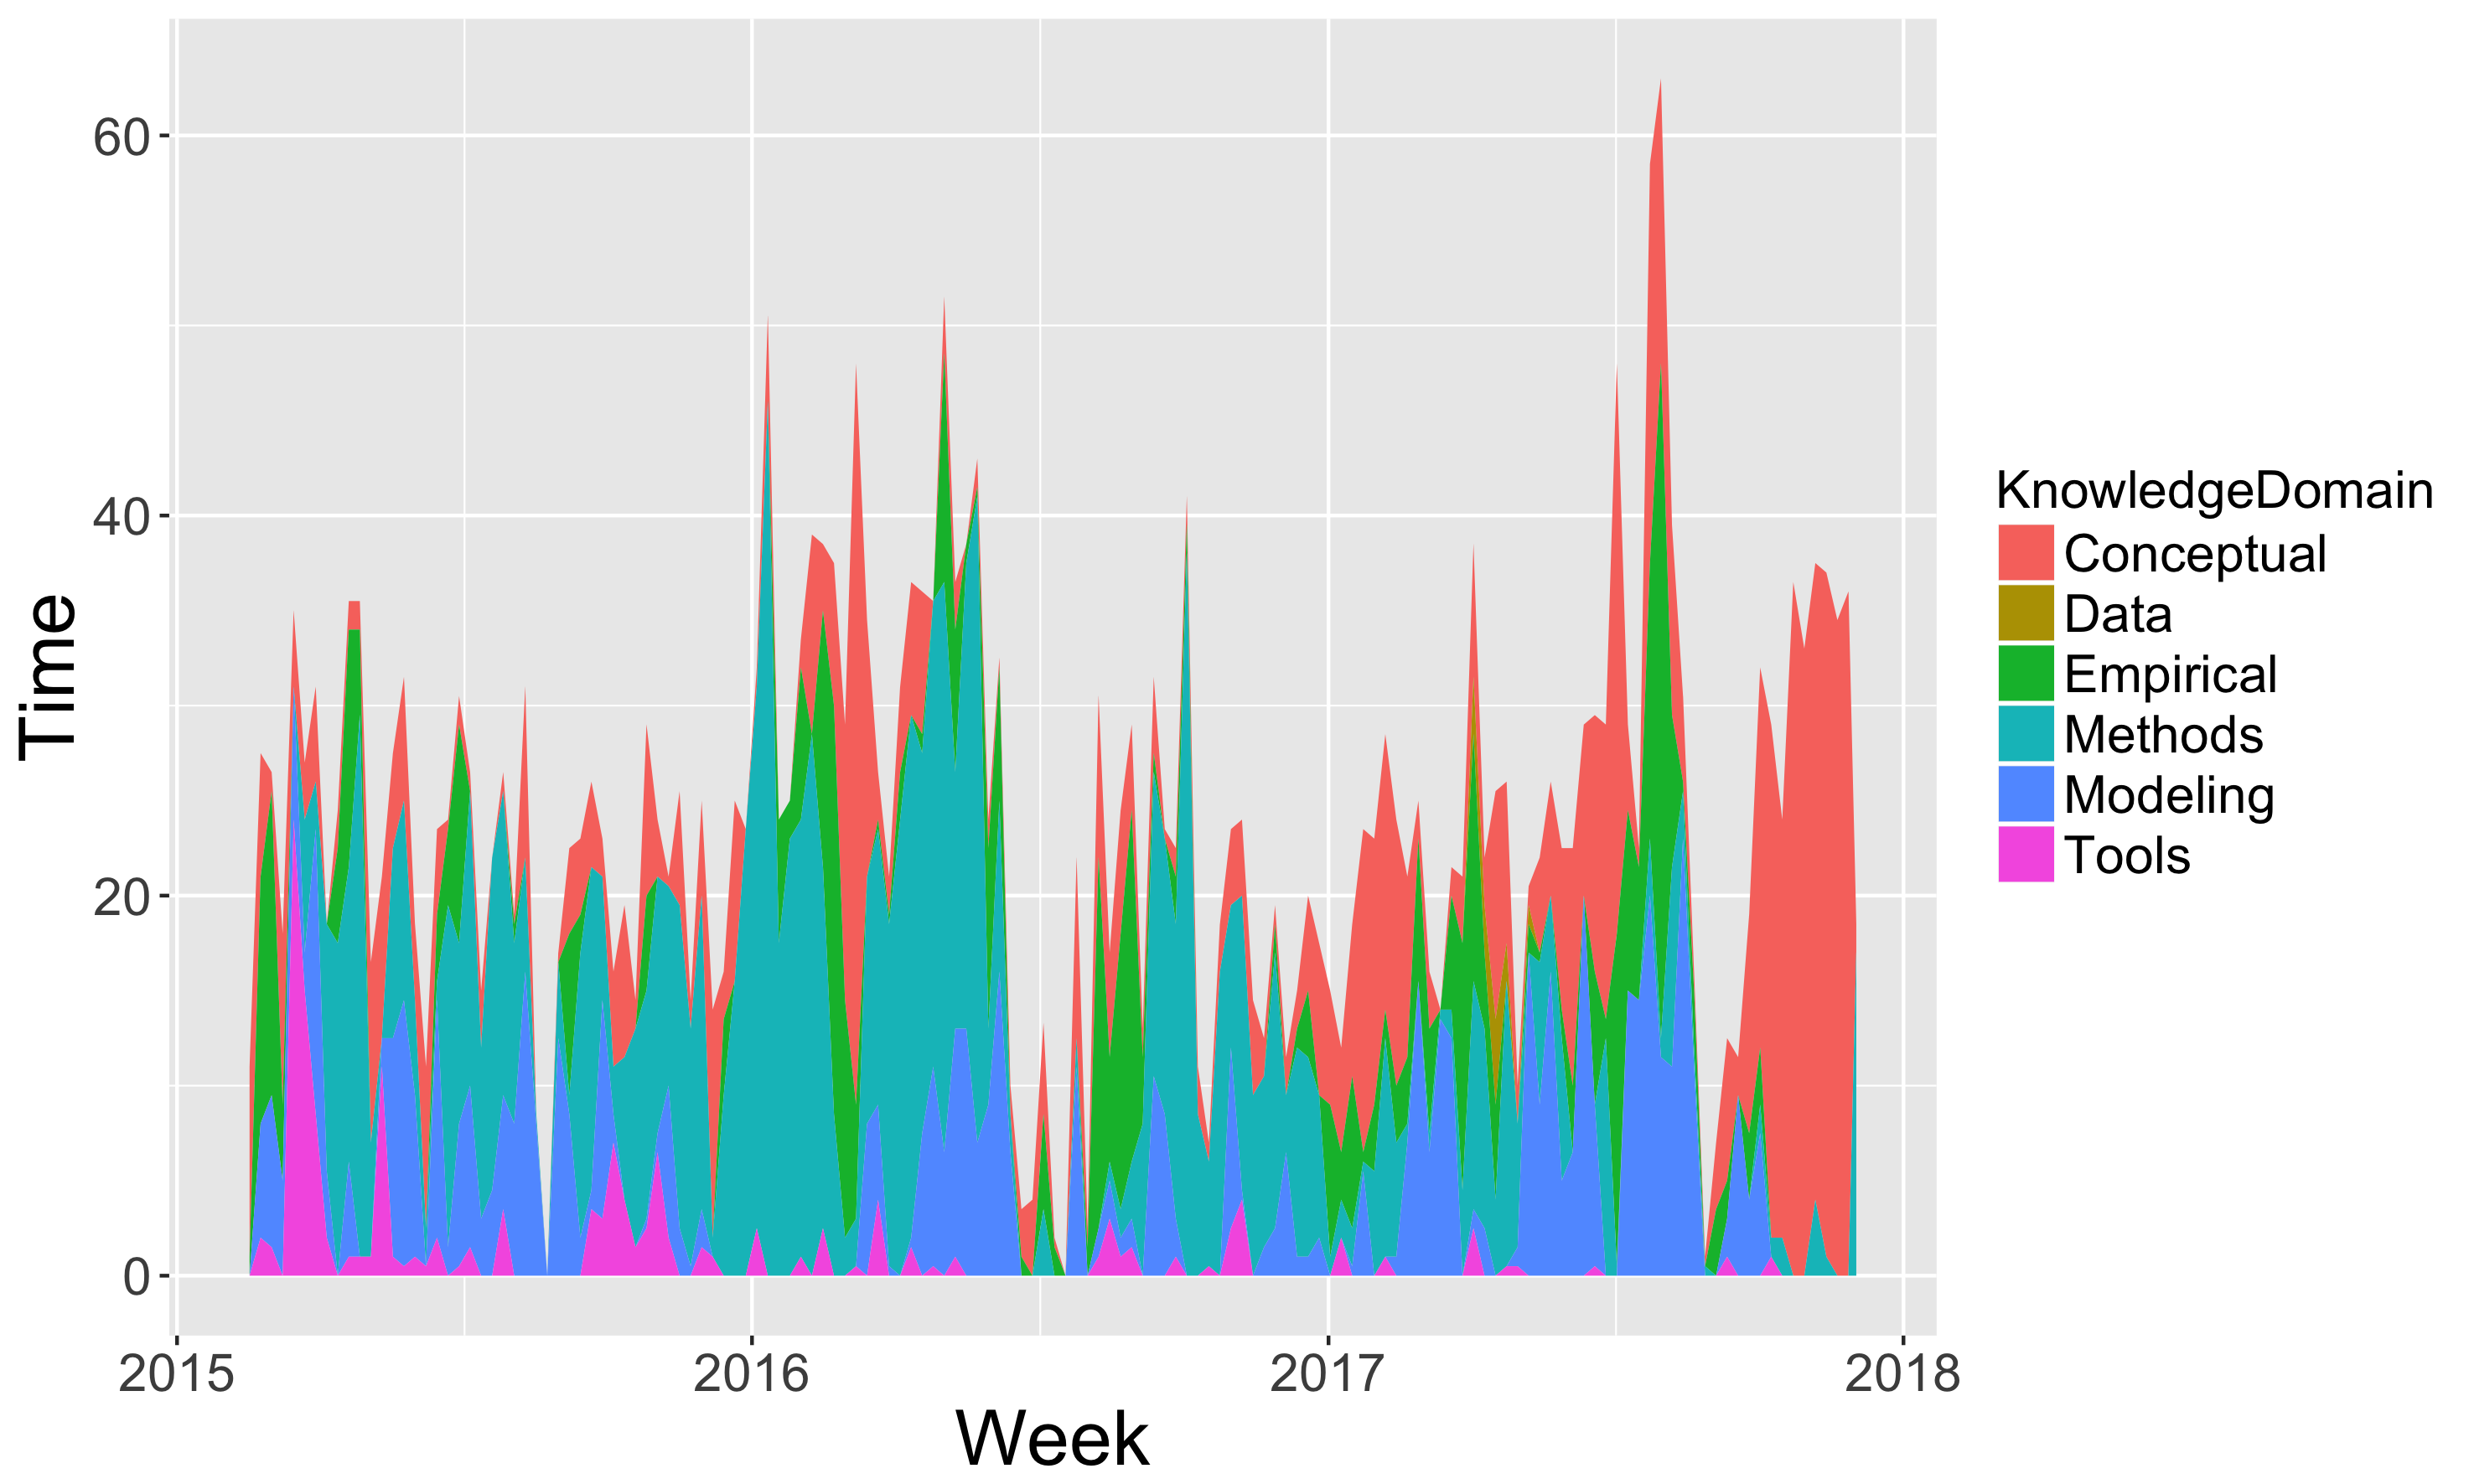
\includegraphics[width=\linewidth]{Figures/Reflexivity/weekly-knowledgedomains.png}
	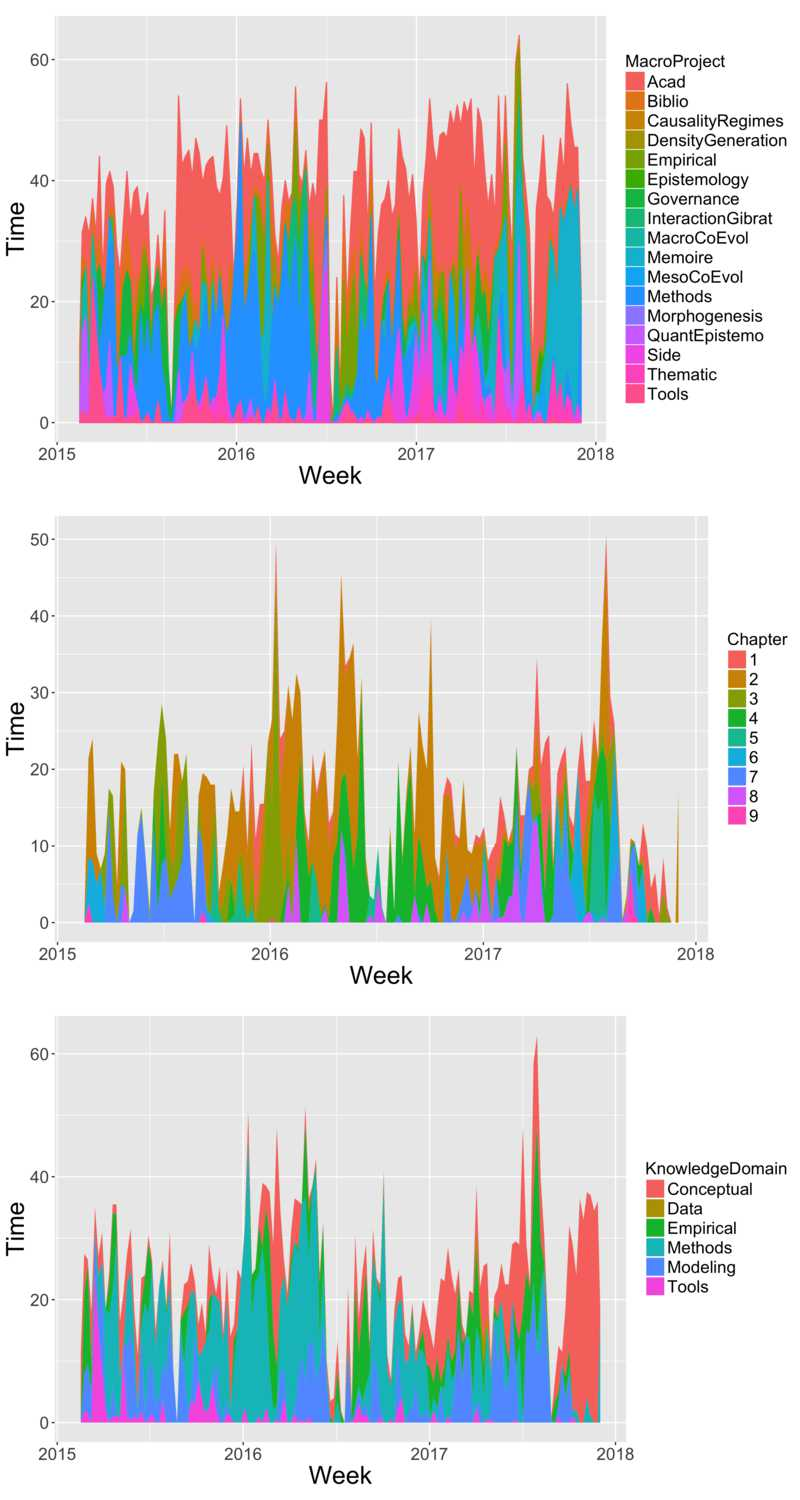
\includegraphics[width=\linewidth,height=\textheight]{Figures/Final/F-reflexivity-time.jpg}
	\appcaption{\textbf{Temporal distribution.}\label{fig:app:reflexivity:time}}{\textbf{Répartition temporelle.} Les temps sont agrégés à la semaine et les aires en couleur donnent la répartition temporelle pour les macro-projets (\textit{première ligne}), les chapitres (\textit{deuxième ligne}) et les domaines de connaissance (\textit{troisième ligne}).\label{fig:app:reflexivity:time}}
\end{figure}
%%%%%%%%%%%%




Il est possible ensuite de construire des graphes d'interaction entre macro-projets ou domaines de connaissance, moyennant des hypothèses simplificatrices.

Un premier indice d'interaction simultanée se base sur l'apparition au même instant. Notons $T_{i,t}$ le temps pour l'entité $i$ (macro-projet ou domaine de connaissance) sur l'unité temporelle $t$ (que nous prendrons à la semaine). La probabilité d'occurence simultanée entre $i$ et $j$ est à l'instant $t$ donnée par $\frac{T_{i,t}T_{j,t}}{\left(\sum_i T_{i,t}\right)^2}$, et nous pouvons les cumuler dans le temps pour avoir un indice d'interaction entre entités :
\[
I_{i,j} = \sum_t \frac{T_{i,t}T_{j,t}}{\left(\sum_i T_{i,t}\right)^2}
\]

La matrice $(I_{i,j})$ permet alors de construire un réseau. Un indice similaire se basant uniquement sur la co-occurrence est donné par

\[
C_{i,j} = \sum_t \mathbbm{1}_{T_{i,t} > 0} \mathbbm{1}_{T_{j,t} > 0}
\]

Nous regardons également des interactions retardées, sous l'hypothèse qu'une entité à l'instant $t$ puisse déclencher celle à l'instant $t+1$, l'indice non symétrique étant alors
\[
\tilde{I}_{i \rightarrow j} = \sum_t \frac{T_{i,t}T_{j,t+1}}{\sum_i T_{i,t}\sum_j T_{j,t+1}}
\]

et le même indice de co-occurence retardé

\[
\tilde{C}_{i\rightarrow j} = \sum_t \mathbbm{1}_{T_{i,t} > 0} \mathbbm{1}_{T_{j,t+1} > 0}
\]


Nous montrons les graphes correspondants pour les macro-projets en Fig.~\ref{fig:app:reflexivity:projects}. Concernant les macro-projets, il apparait que le coeur du réseau de co-occurrence simultanée est constitué par la bibliographie, la vie académique et les méthodes : ces éléments sont quasiment présent à chaque instant et structurent le reste de la recherche. Ensuite, les différents projets thématiques peuvent être menés relativement indépendamment, et gravitent à la périphérie du réseau. Avec le graphe dirigé des interactions retardées, il n'est guère possible de tirer une information supplémentaire, les flux étant quasi-symétriques : soit l'agrégation à la semaine n'est pas pertinente soit le délai peut être différent, soit il y a effectivement réciprocité, cette dernière hypothèse étant crédible vu l'intrication des projets.


%%%%%%%%%%%%
\begin{figure}
	%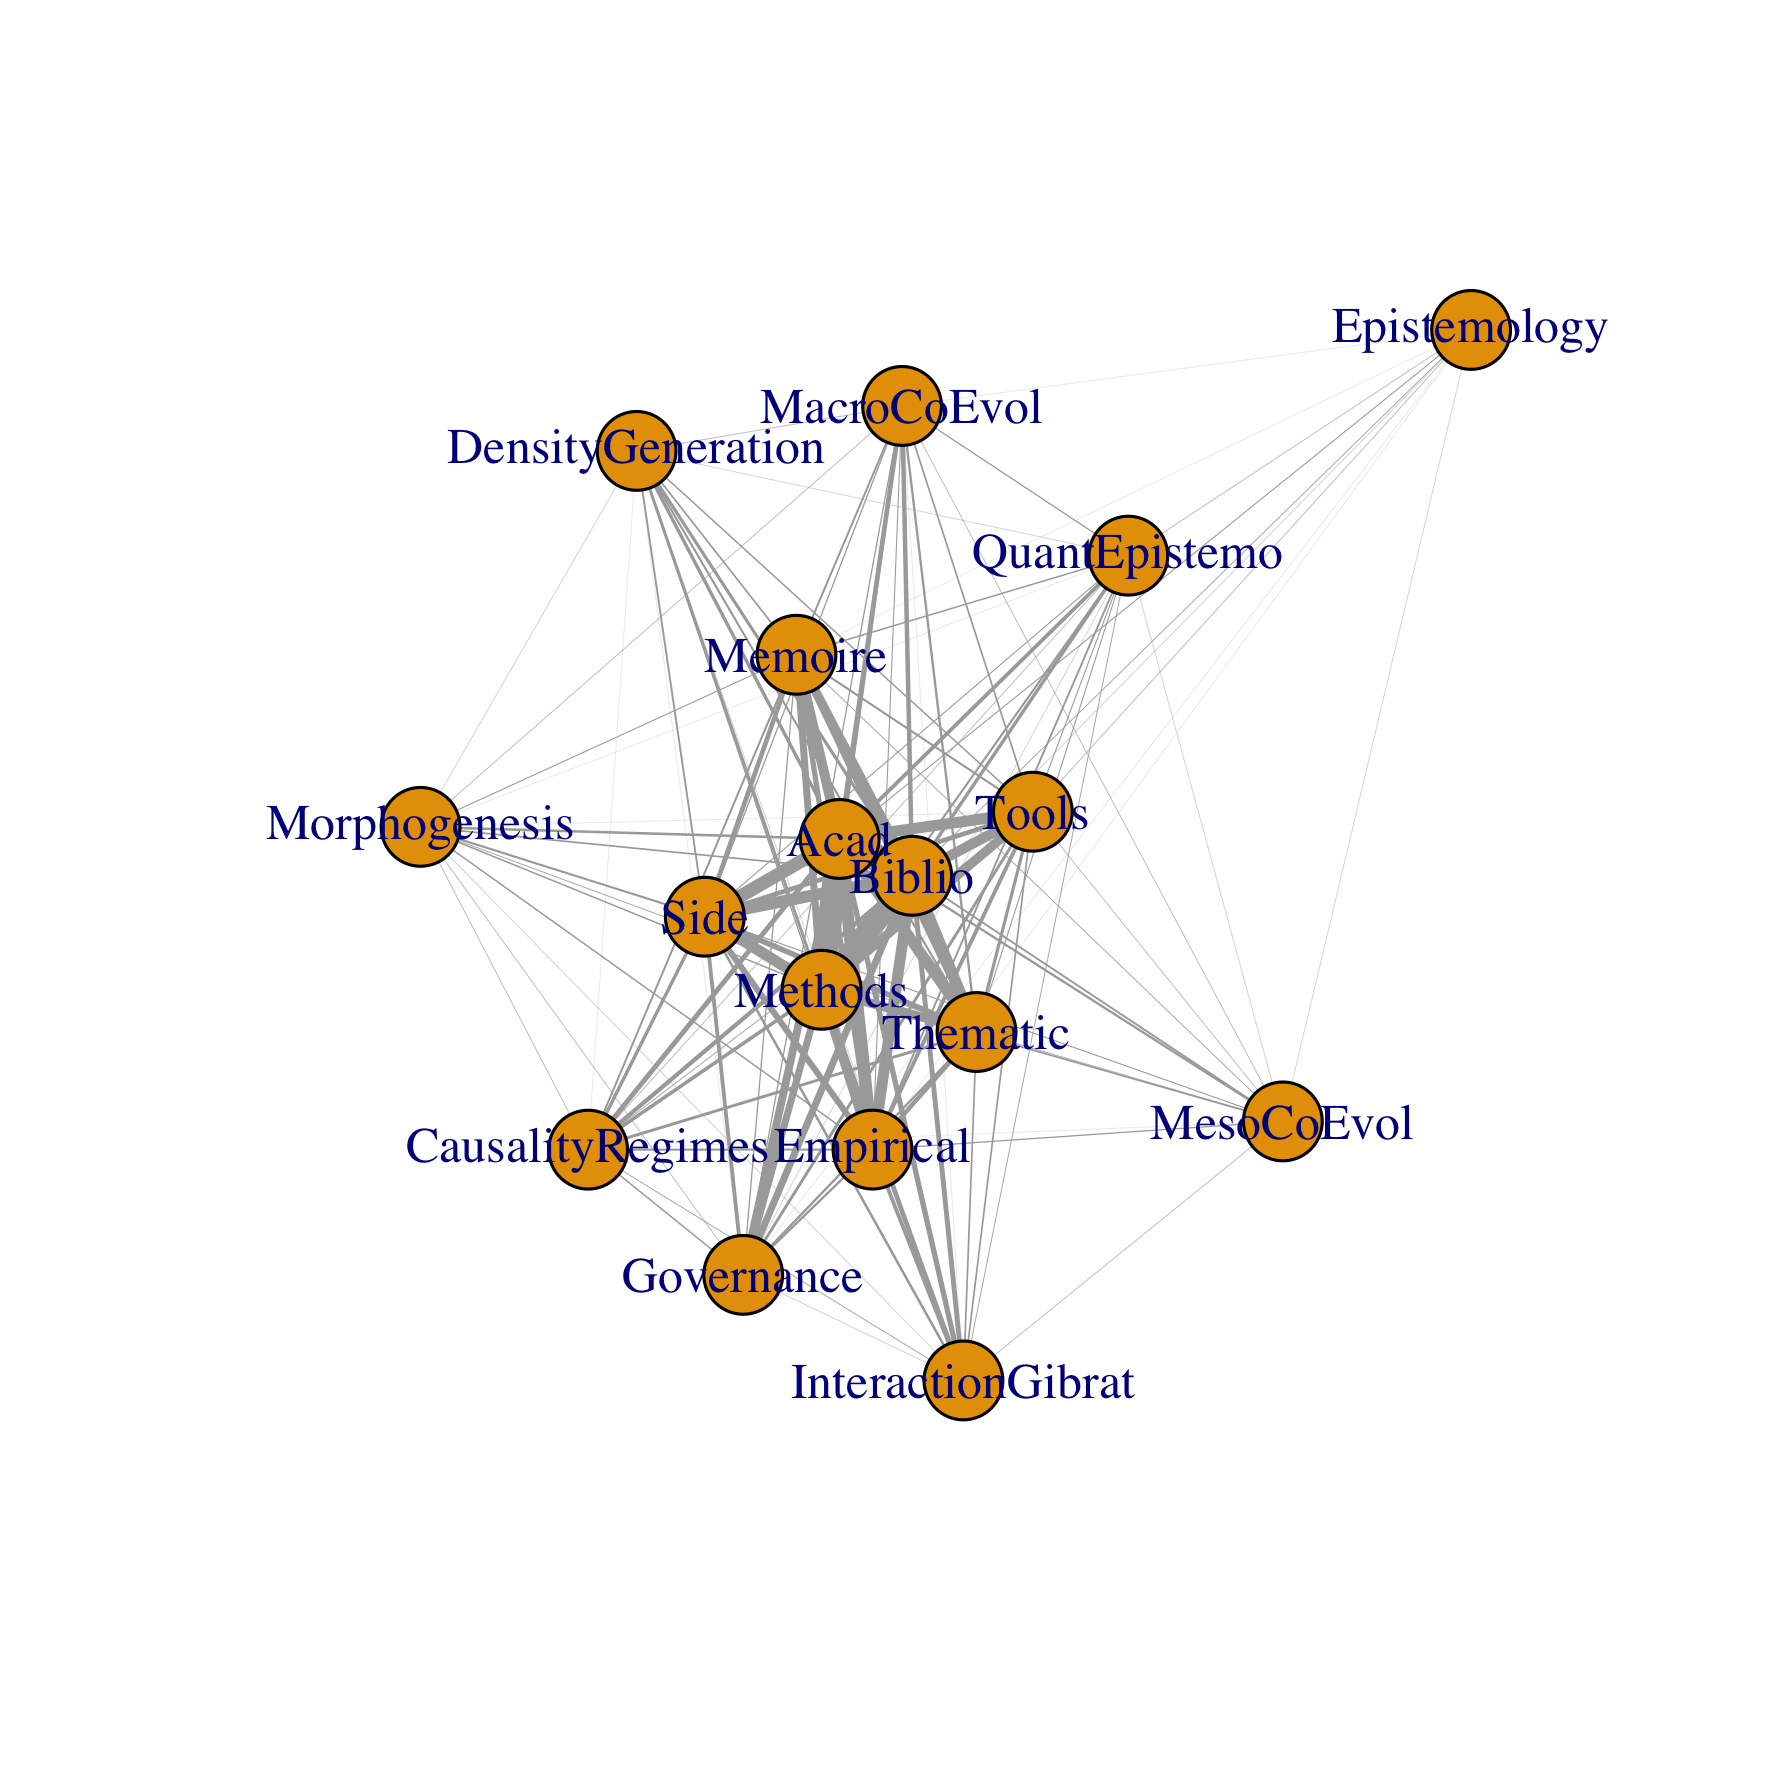
\includegraphics[width=0.49\linewidth]{Figures/Reflexivity/graph-projects-cooccs.png}
	%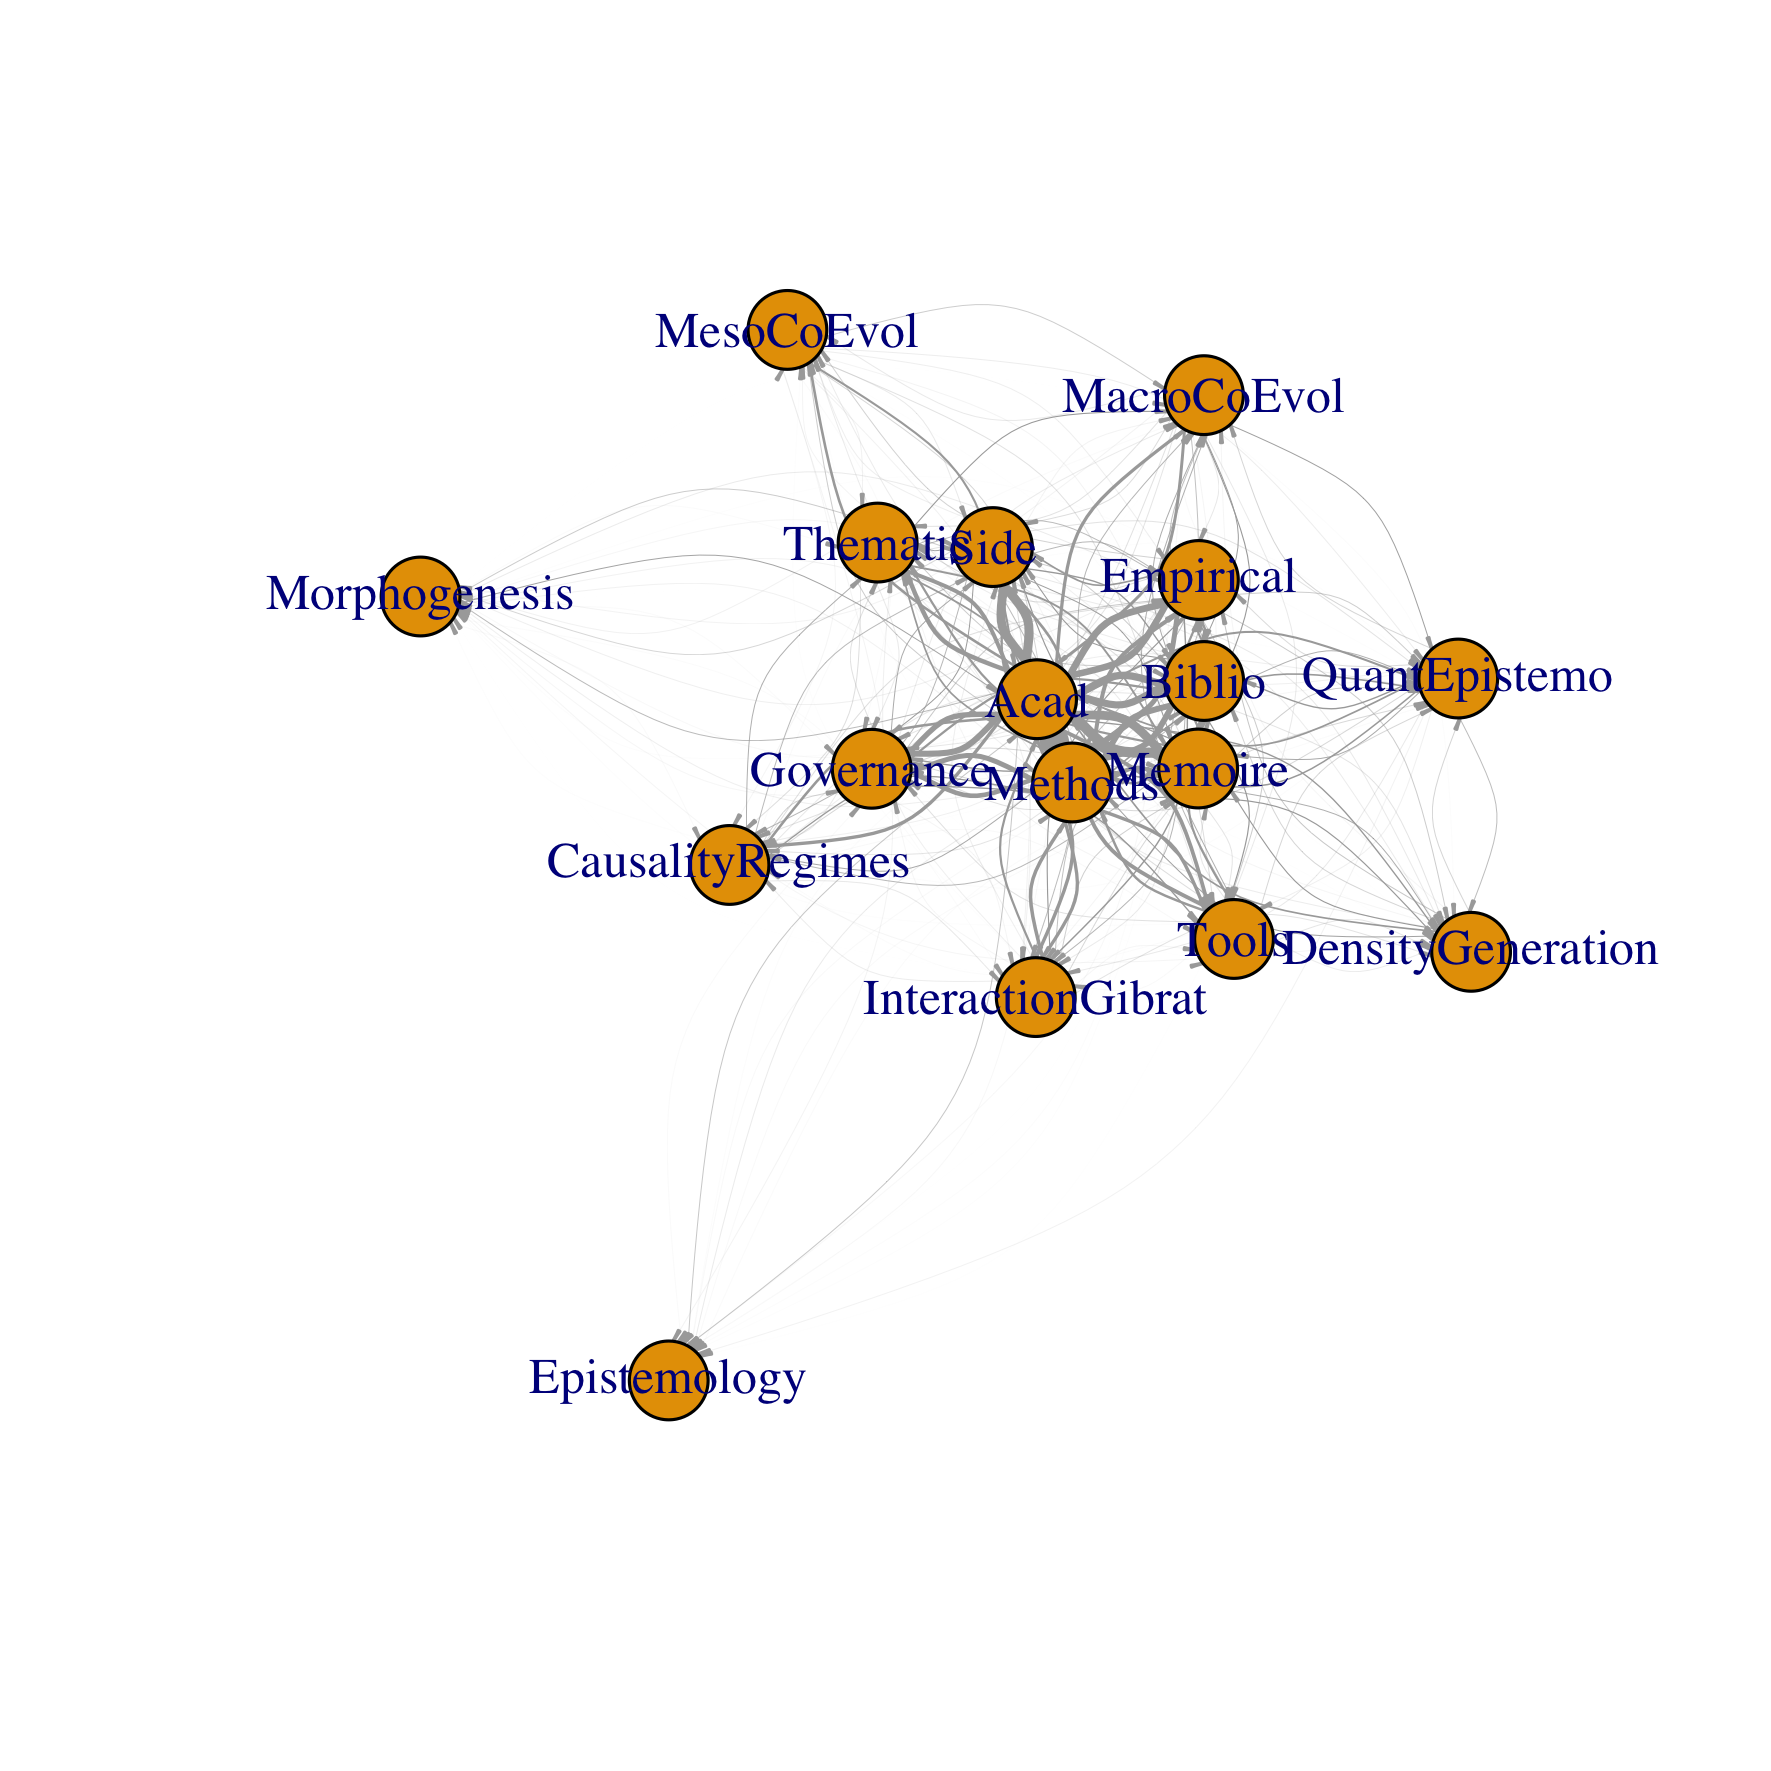
\includegraphics[width=0.49\linewidth]{Figures/Reflexivity/graph-projects-laggedflow.png}
	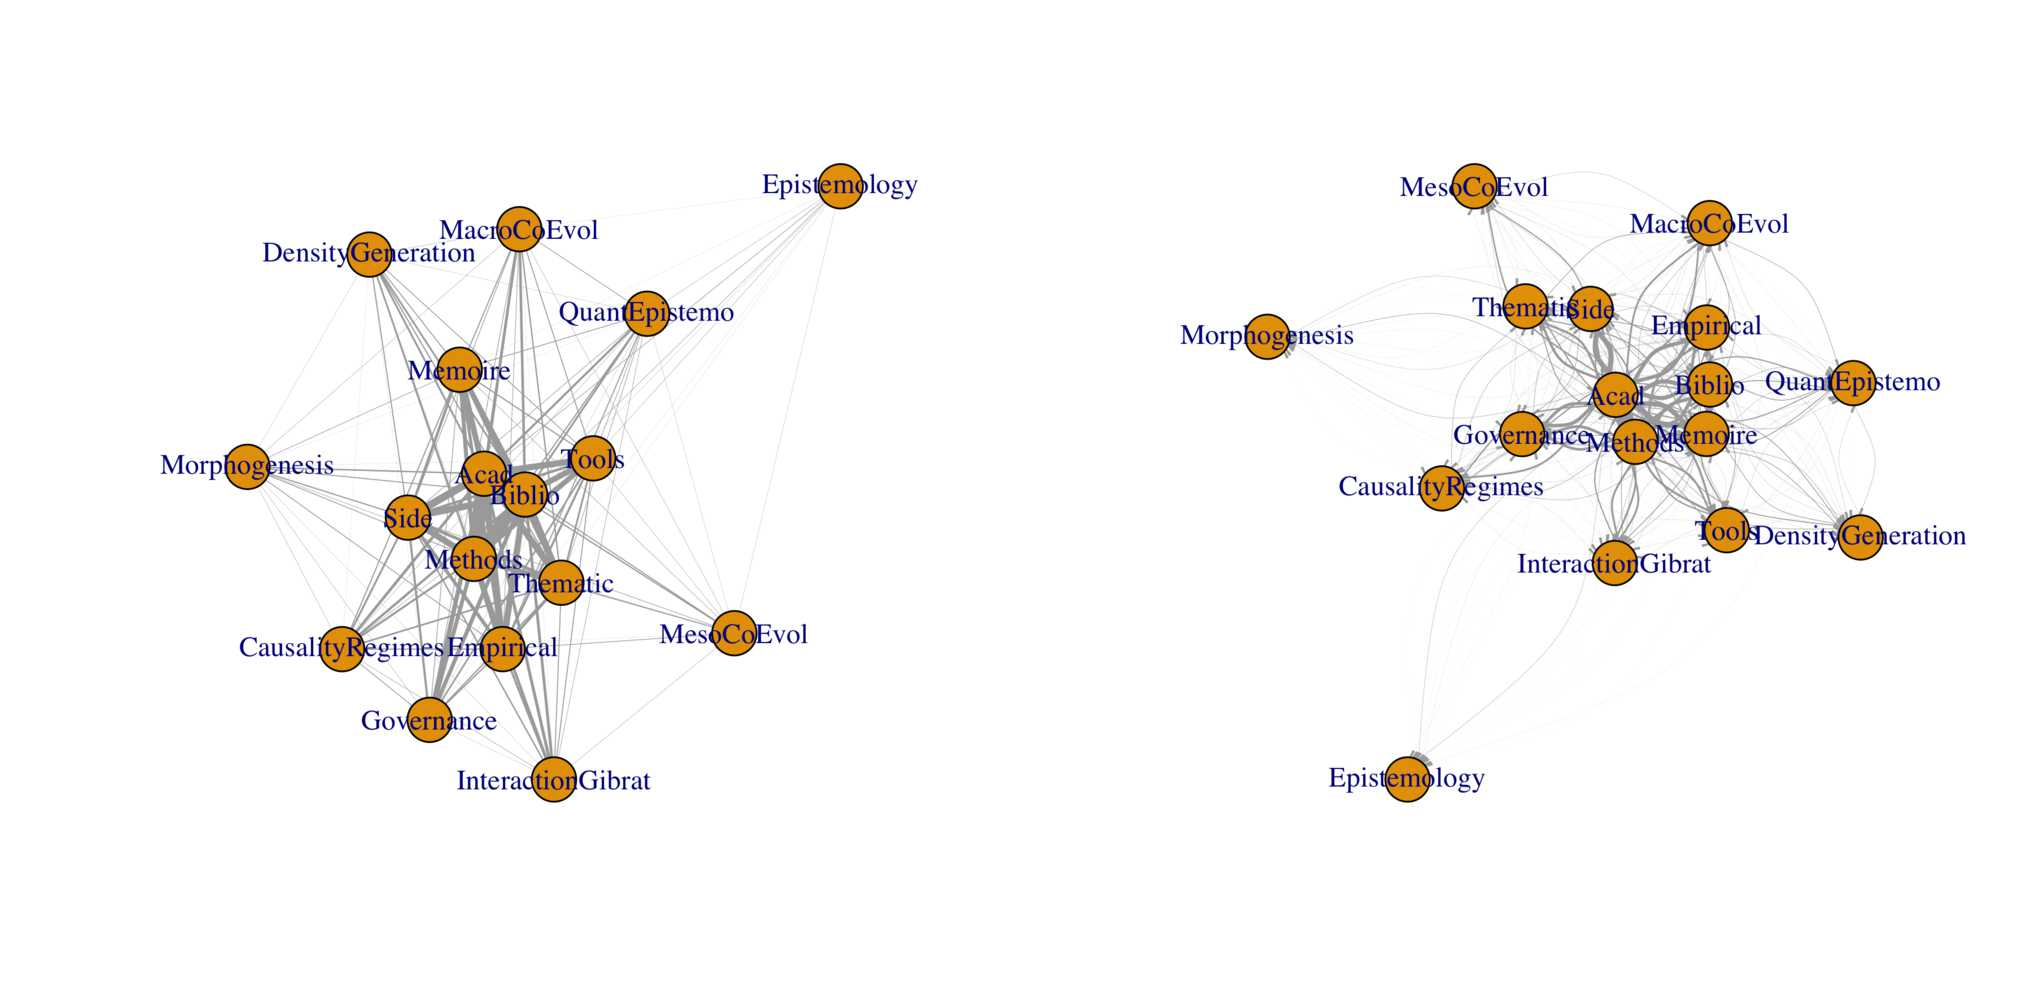
\includegraphics[width=\linewidth]{Figures/Final/F-reflexivity-projects.jpg}
	\appcaption{\textbf{Interaction networks between projects}\label{fig:app:reflexivity:projects}}{\textbf{Graphes d'interaction entre macro-projets.} (\textit{Gauche}) Graphe d'interaction simultanée par co-occurrence, donné par la matrice d'adjacence $C_{i,j}$ ; (\textit{Droite}) Graphe d'interaction retardée, donné ici par les flux $\tilde{I}_{i \rightarrow j}$. \label{fig:app:reflexivity:projects}}
\end{figure}
%%%%%%%%%%%%


Les graphes pour les domaines de connaissance est donné en Fig.~\ref{fig:app:reflexivity:kd}. Outre que les données sont relativement périphériques, ce qui est attendu vu leur faible importance et leur intégration au sein d'autres projets, nous n'observons pas de motifs particuliers dans ces graphes : l'ensemble des domaines est mobilisé à la plupart des instants. Il y a également l'ensemble des relations réciproques dans le graphe dirigé, ce qui suggère éventuellement une co-évolution entre les domaines de connaissance, ce que nous allons vérifier par la suite.

%%%%%%%%%%%%
\begin{figure}
	%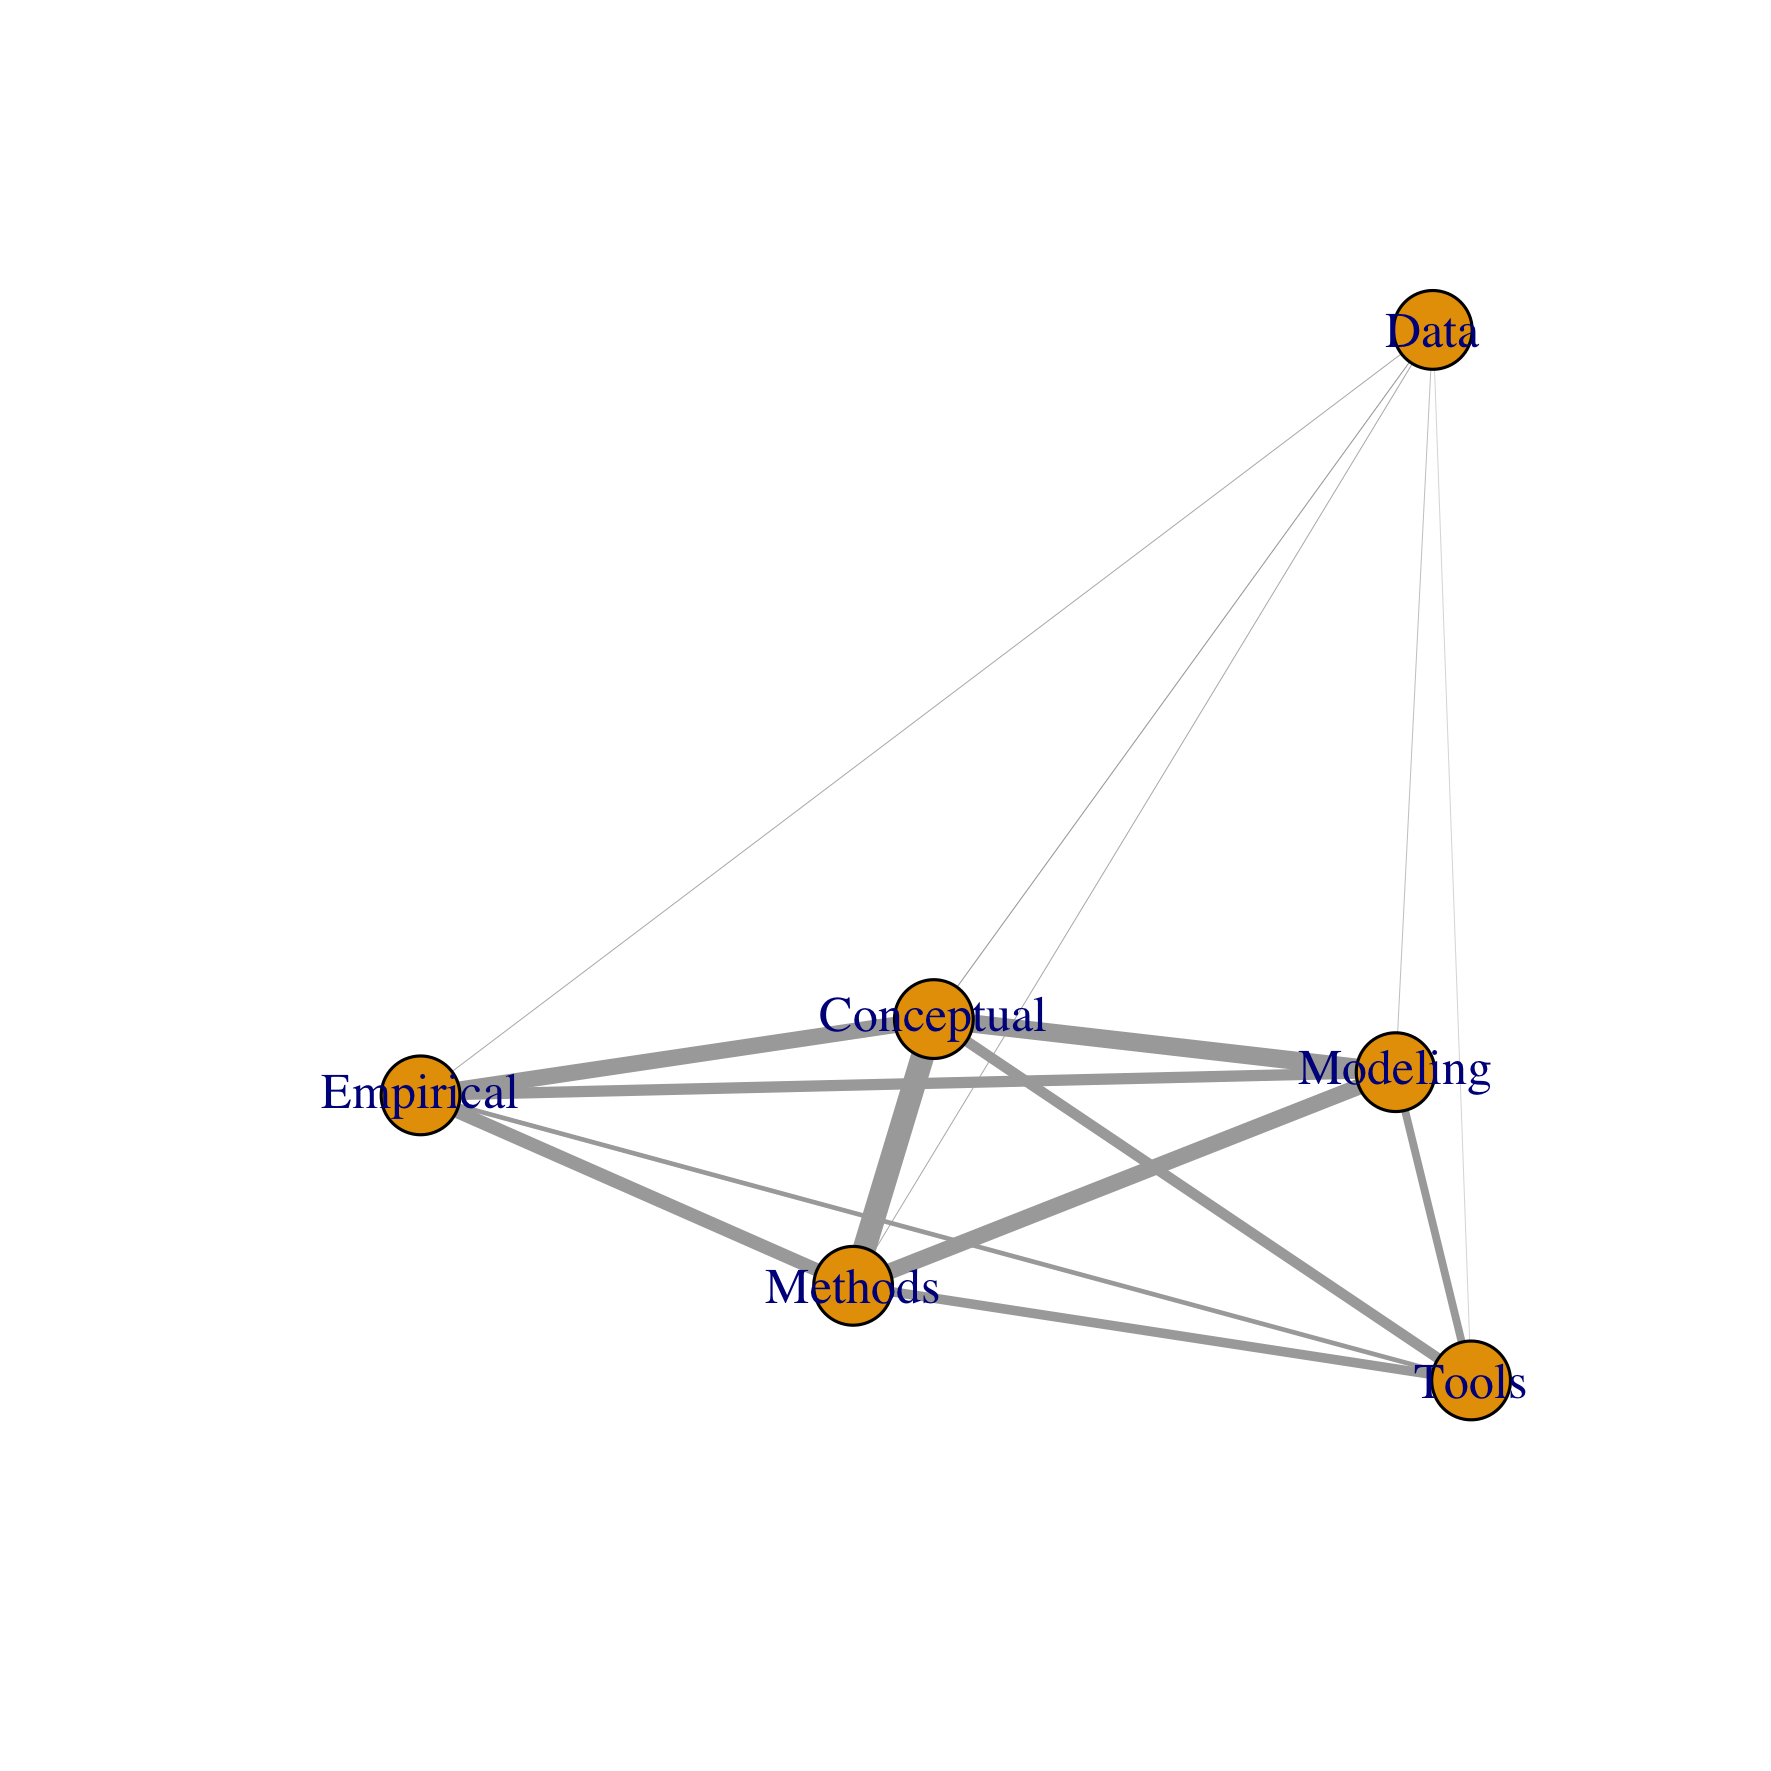
\includegraphics[width=0.49\linewidth]{Figures/Reflexivity/graph-kd-cooccs.png}
	%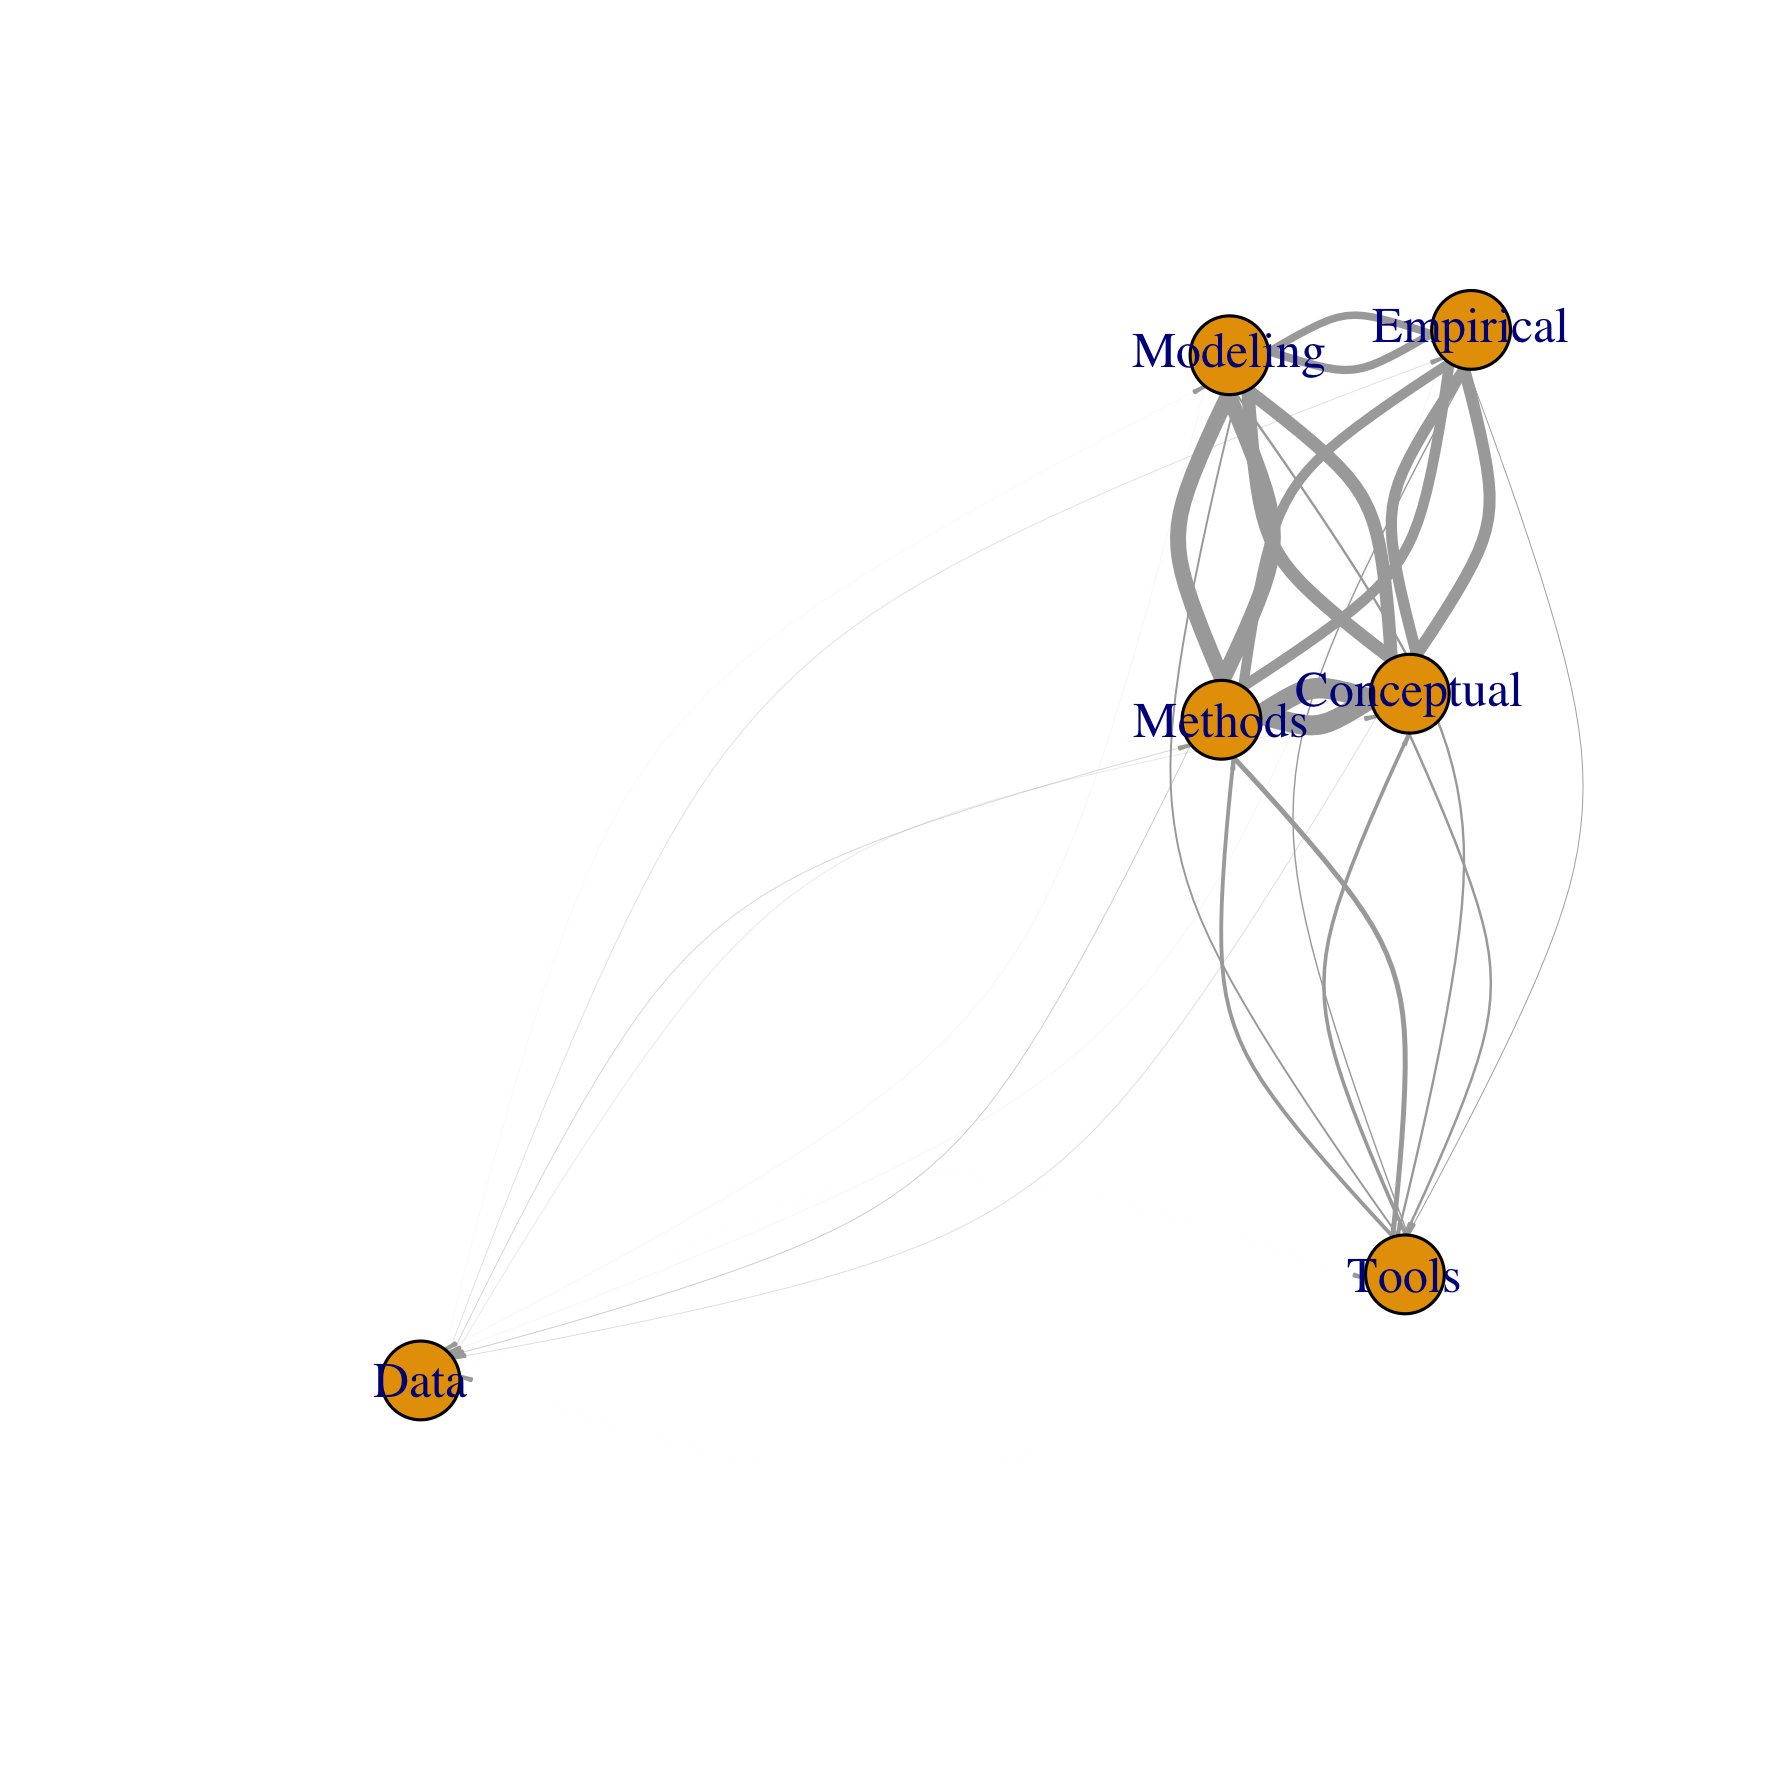
\includegraphics[width=0.49\linewidth]{Figures/Reflexivity/graph-kd-laggedflow.png}
	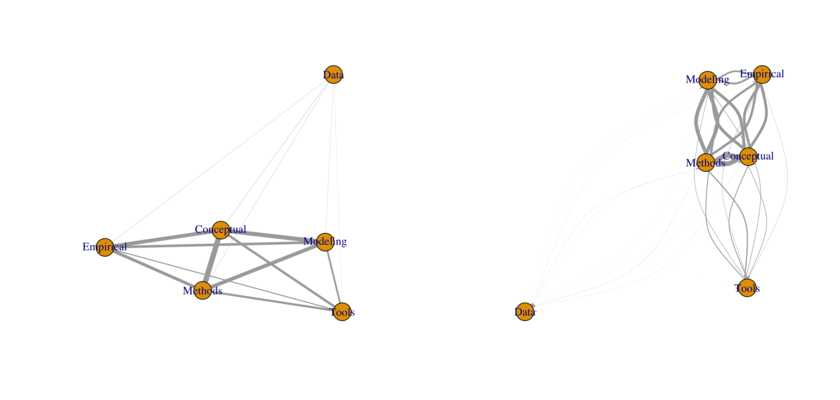
\includegraphics[width=\linewidth]{Figures/Final/F-reflexivity-kd.jpg}
	\appcaption{\textbf{Interaction networks between knowledge domains.}\label{fig:app:reflexivity:kd}}{\textbf{Graphes d'interaction entre domaines de connaissance.} (\textit{Gauche}) Graphe d'interaction simultanée par co-occurrence ; (\textit{Droite}) Graphe d'interaction retardée.\label{fig:app:reflexivity:kd}}
\end{figure}
%%%%%%%%%%%%



% kddata%>%group_by(KnowledgeDomain)%>%summarise(time=sum(time))
%  KnowledgeDomain   time
%           <fctr>  <dbl>
%1      Conceptual 1003.8
%2            Data   13.0
%3       Empirical  496.0
%4         Methods 1256.0
%5        Modeling  656.0
%6           Tools  147.0


Nous estimons pour chaque couple de domaine de connaissance $i,j$ (hors du domaine données qui ne cumule que 13h au total donc trop peu de variations pour estimer une corrélation) les corrélations retardées entre les différences $\rhob{\Delta T_{i,t-\tau}}{T_{j,t}}$ pour $-4 \leq \tau 4$ (délai maximal d'un mois). Nous conservons les corrélations si $p<0.05$ et sélectionnons la corrélation absolue maximale pour chaque couple de variable si elle existe.

%%%%%%%%%%%%%%
\begin{figure}
	%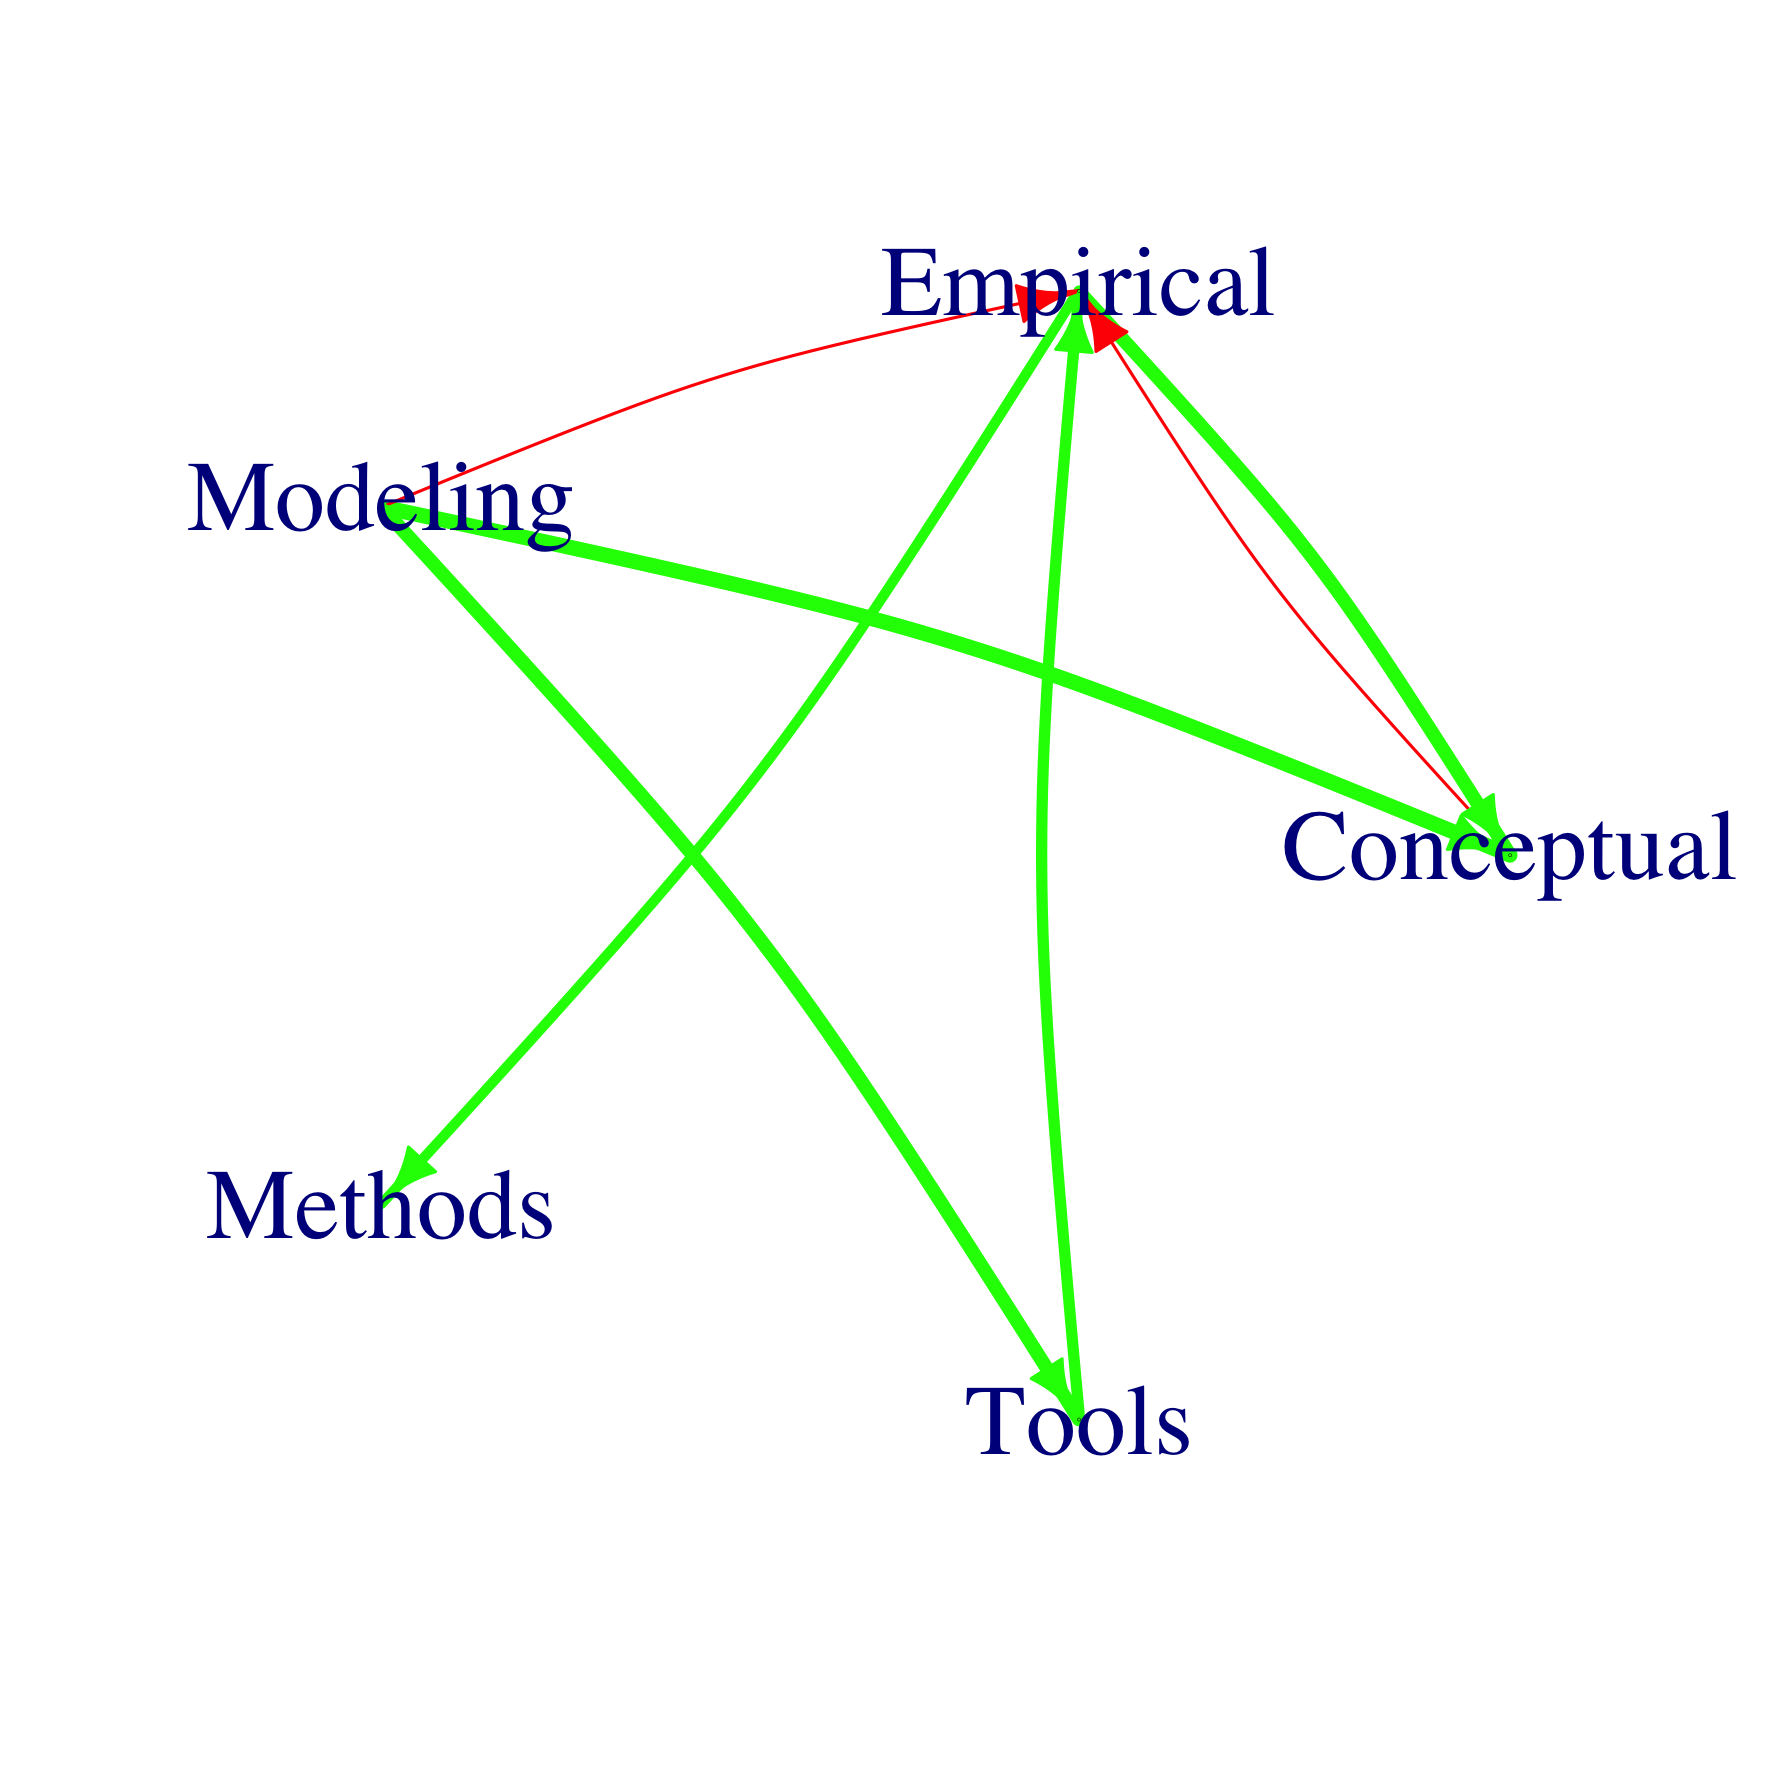
\includegraphics[width=\linewidth]{Figures/Reflexivity/laggedcorrs.png}
	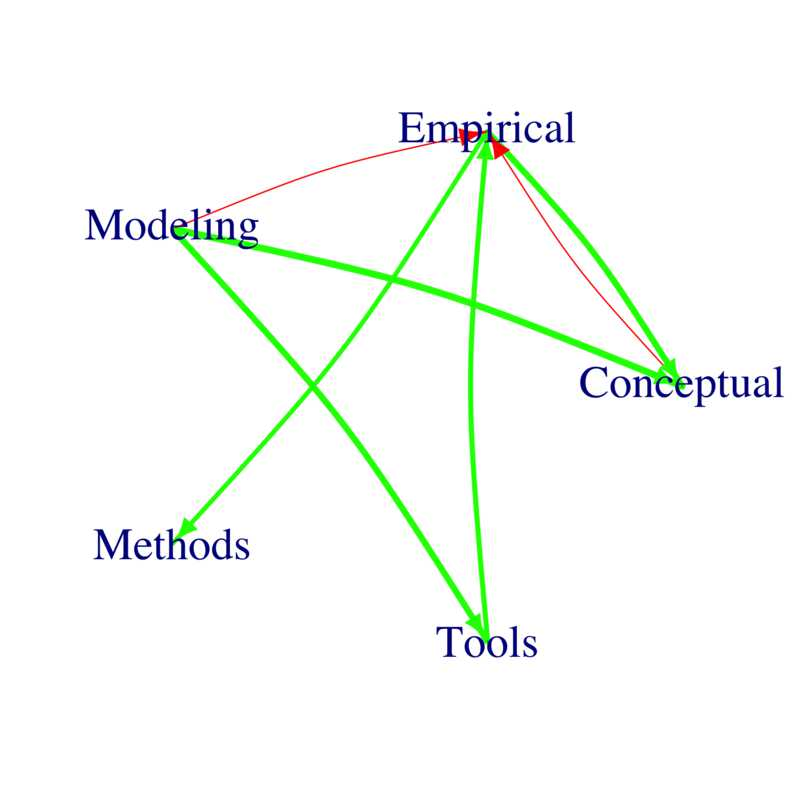
\includegraphics[width=\linewidth]{Figures/Final/F-reflexivity-laggedcorrs.jpg}
	\appcaption{\label{fig:app:reflexivity:laggedcorrs}}{\textbf{Graphe de corrélations retardées entre domaines de connaissances.} La couleur donne le signe de la corrélation (vert : positif, rouge : négatif) et l'épaisseur du lien sa valeur. Les liens existent si et seulement si $p<0.05$ pour un test de Fisher.\label{fig:app:reflexivity:laggedcorrs}}
\end{figure}
%%%%%%%%%%%%%%


Le graphe des corrélations retardées est donné en Fig.~\ref{fig:app:reflexivity:laggedcorrs}. Il existe un certain nombre de liens significatifs, et même une relation circulaire entre empirique et conceptuel, c'est-à-dire une co-évolution à proprement parler entre ces domaines. La modélisation et l'empirique induisent des travaux dans le domaine conceptuel, ce qui peut s'interpréter comme une induction des théories. Par contre, le conceptuel diminue l'empirique, ce qui pourrait être symptôme d'une trop grande déconnexion avec le concret parfois.

Ainsi, même si ces résultats sont bien sûr à prendre avec précaution vu les biais intrinsèques aux données (difficulté de donner un label, réduction au sein de projets, etc.), nous suggérons une intrication des domaines de connaissance et une co-évolution pour certains. Cela peut être mis en écho avec l'hypothèse fondamentale du cadre de connaissance développé en~\ref{sec:knowledgeframework}, qui implique qu'une connaissance complexe nécessite co-évolution des domaines. Enfin, l'application des propres outils de notre travail à lui-même suggère une dimension hologrammatique~\cite{morin1986methode}, rappelant le lien entre complexité et production de connaissance suggéré en~\ref{sec:epistemology}. 



\stars



%%%%%%%
%% -- on hold --

%%%%%%%%%%%%
%\subsection{Concept maps}{Cartographie des concepts}

%concept maps : \cite{novak2008theory}

% faire un graphe des concepts ; compare to semantic network of concepts in Gödel Escher Bach.




% To clarify the plan : Plan (of course) ; diagram for plan ; and dependence tree for parts/sections
% --> en intro


%  ``Meta-conclusion''
%  -> should also include reading graph / possible paths





